\documentclass[reprint,english,notitlepage]{revtex4-1}  % defines the basic parameters of the document

% if you want a single-column, remove reprint

% allows special characters (including æøå)
\usepackage[utf8]{inputenc}
\usepackage[english]{babel}

%% note that you may need to download some of these packages manually, it depends on your setup.
%% I recommend downloading TeXMaker, because it includes a large library of the most common packages.

\usepackage{physics,amssymb}  % mathematical symbols (physics imports amsmath)
\usepackage{graphicx}         % include graphics such as plots
\usepackage{xcolor}           % set colors
\usepackage{hyperref}         % automagic cross-referencing (this is GODLIKE)
\usepackage{tikz}             % draw figures manually
\usepackage{listings}         % display code
\usepackage{subfigure}        % imports a lot of cool and useful figure commands
\usepackage{cprotect}
\usepackage{float}


% defines the color of hyperref objects
% Blending two colors:  blue!80!black  =  80% blue and 20% black
\hypersetup{ % this is just my personal choice, feel free to change things
    colorlinks,
    linkcolor={red!50!black},
    citecolor={blue!50!black},
    urlcolor={blue!80!black}}
%
%% Defines the style of the programming listing
%% This is actually my personal template, go ahead and change stuff if you want
\lstnewenvironment{python}{
	\lstset{ %
		inputpath=,
		backgroundcolor=\color{white!88!black},
		basicstyle={\ttfamily\scriptsize},
		commentstyle=\color{magenta},
		language=Python,
		morekeywords={True,False},
		tabsize=4,
		stringstyle=\color{green!55!black},
		frame=single,
		keywordstyle=\color{blue},
		showstringspaces=false,
		columns=fullflexible,
		keepspaces=true}
}{}

\lstnewenvironment{cpp}{
	\lstset{ %
		inputpath=,
		backgroundcolor=\color{white!88!black},
		basicstyle={\ttfamily\scriptsize},
		commentstyle=\color{magenta},
		language=C++,
		morekeywords={True,False},
		tabsize=4,
		stringstyle=\color{green!55!black},
		frame=single,
		keywordstyle=\color{blue},
		showstringspaces=false,
		columns=fullflexible,
		keepspaces=true}
}{}

\lstset{literate=
  {á}{{\'a}}1 {é}{{\'e}}1 {í}{{\'i}}1 {ó}{{\'o}}1 {ú}{{\'u}}1
  {Á}{{\'A}}1 {É}{{\'E}}1 {Í}{{\'I}}1 {Ó}{{\'O}}1 {Ú}{{\'U}}1
  {à}{{\`a}}1 {è}{{\`e}}1 {ì}{{\`i}}1 {ò}{{\`o}}1 {ù}{{\`u}}1
  {À}{{\`A}}1 {È}{{\'E}}1 {Ì}{{\`I}}1 {Ò}{{\`O}}1 {Ù}{{\`U}}1
  {ä}{{\"a}}1 {ë}{{\"e}}1 {ï}{{\"i}}1 {ö}{{\"o}}1 {ü}{{\"u}}1
  {Ä}{{\"A}}1 {Ë}{{\"E}}1 {Ï}{{\"I}}1 {Ö}{{\"O}}1 {Ü}{{\"U}}1
  {â}{{\^a}}1 {ê}{{\^e}}1 {î}{{\^i}}1 {ô}{{\^o}}1 {û}{{\^u}}1
  {Â}{{\^A}}1 {Ê}{{\^E}}1 {Î}{{\^I}}1 {Ô}{{\^O}}1 {Û}{{\^U}}1
  {œ}{{\oe}}1 {Œ}{{\OE}}1 {æ}{{\ae}}1 {Æ}{{\AE}}1 {ß}{{\ss}}1
  {ű}{{\H{u}}}1 {Ű}{{\H{U}}}1 {ő}{{\H{o}}}1 {Ő}{{\H{O}}}1
  {ç}{{\c c}}1 {Ç}{{\c C}}1 {ø}{{\o}}1 {å}{{\r a}}1 {Å}{{\r A}}1
  {€}{{\euro}}1 {£}{{\pounds}}1 {«}{{\guillemotleft}}1
  {»}{{\guillemotright}}1 {ñ}{{\~n}}1 {Ñ}{{\~N}}1 {¿}{{?`}}1
}



\usepackage{thmtools}
\DeclareMathOperator{\nullspace}{Nul}
\DeclareMathOperator{\collspace}{Col}
\DeclareMathOperator{\rref}{Rref}
%%\DeclareMathOperator{\dim}{Dim}

 % "meq": must be equal
\newcommand{\meq}{\overset{!}{=}}
\newcommand\numberthis{\addtocounter{equation}{1}\tag{\theequation}}

\newcommand{\R}{\mathbb{R}}
\newcommand*\Heq{\ensuremath{\overset{\kern2pt L'H}{=}}}
\usepackage{bm}
\newcommand{\uveci}{{\bm{\hat{\textnormal{\bfseries\i}}}}}
\newcommand{\uvecj}{{\bm{\hat{\textnormal{\bfseries\j}}}}}
\DeclareRobustCommand{\uvec}[1]{{%
  \ifcsname uvec#1\endcsname
     \csname uvec#1\endcsname
   \else
    \bm{\hat{\mathbf{#1}}}%
   \fi
}}
\usepackage[binary-units=true]{siunitx}

\makeatletter
\newcommand*{\balancecolsandclearpage}{%
  \close@column@grid
  \cleardoublepage
  \twocolumngrid
}
\makeatother

\newcounter{subproject}
\renewcommand{\thesubproject}{\alph{subproject}}
\newenvironment{subproj}{
\begin{description}
	\item[\refstepcounter{subproject}(\thesubproject)]
}{\end{description}}


\begin{document}
\title{On the numerical simulation of the diffusion equation in 1D with explicit and implicit schemes, and the 2D simulation of heat diffusion in the litosphere using Jacobi's iterative method}   % self-explanatory
\author{Eivind Støland, Anders P. Åsbø}               % self-explanatory
\date{\today}                             % self-explanatory
\noaffiliation                            % ignore this

\begin{abstract}
Abstract
\end{abstract}

\maketitle                                % creates the title, author, date


\tableofcontents

\section{Introduction} \label{sec:introduction}


\clearpage

\section{Formalism} \label{sec:formalism}

\subsection{Diffusion equation} \label{sec:formalism_diffusion_equation}

By scaling variables, we can write the general diffusion equation as follows:

\begin{align*}
\nabla^2 u(\vec{r},t) = \frac{\partial u(\vec{r},t)}{\partial t} \, , \numberthis \label{eq:3D_diff_eq}
\end{align*}

where $\nabla$ is the spatial derivative, $\vec{r}$ a vector containing spatial coordinates, $t$ is time, and what $u$ is depends on which system we are looking it in particular. This equation can be used to model several physical phenomena, such as mixing of particles, and perhaps most famously heat conductance through the heat equation:

\begin{align*}
\frac{k}{c_p \rho} \nabla^2 T(\vec{r},t) = \frac{\partial T (\vec{r},t)}{\partial t} \, , \numberthis \label{eq:heat_equation_general}
\end{align*}

where $k$ is the thermal conductivity, $c_p$ is the specific heat, $\rho$ is the density of the material, and $T$ is the temperature gradient. This is an equation that we will use, and so we need to scale it. Firstly we can define the diffusion constant $D = c_p \rho / k$. This means we can write the heat equation as:

\begin{align*}
\nabla^2 T(\vec{r},t) &= D \frac{\partial T(\vec{r},t)}{\partial t}
\end{align*}

Now we define the spatial coordinate vector $\vec{r} = \alpha \hat{\vec{r}}$, where $\alpha$ is an arbitrary constant. Substituting this affects the spatial derivative such that the equation now reads:

\begin{align*}
\frac{1}{\alpha^2} \nabla^2 T(\vec{r},t) &= D \frac{\partial T(\vec{r},t)}{\partial t}
\end{align*}  

As $\alpha$ is an arbitrary constant we can now choose it such that $D = 1/\alpha^2$. The equation then reads:

\begin{align*}
\nabla^2 T(\vec{r},t) &= \frac{\partial T(\vec{r},t)}{\partial t} \, ,
\end{align*}

which is just the general diffusion equation we have listed earlier, with $u$ exchanged for $T$. In other words, if we can solve the general diffusion equation, we can also solve the heat equation.

When solving the diffusion equation numerically it is common to scale the spatial coordinates so that $x,y,z \in [0,1]$ if we are using cartesian coordinates. As long as we are looking at a square system, this does not cause any problems for the method outlined earlier, as we can easily model other choices of limits by adding a constant to the spatial coordinate and correctly choosing $\alpha$. We also assume that the initial state and the boundary conditions are known: 

\begin{align*}
u(x,y,z,0) &= f(x,y,z) \\
u(0,y,z,t) &= g(y,z,t) \\
u(1,y,z,t) &= h(y,z,t) \\
u(x,0,z,t) &= k(x,z,t) \\
\vdots 
\end{align*}

and so on for the other coordinates as well.
 
In the following sections we will look at solutions to the diffusion equation in 1D and 2D both numerically and analytically.




\subsection{Analytical solution of diffusion equation in one dimension} \label{sec:formalism_1D_diff_eq_analytical}

In order to find a solution we need to make some assumptions based on the initial and boundary conditions. We assume that:

\begin{align*}
u(x,0) = g(x) \quad 0 < x < L
\end{align*}

and:

\begin{align*}
u(0,t) = u(L,t) = 0 \quad t \geq 0
\end{align*}

The equation wish to solve is the general diffusion equation in one dimension:

\begin{align*}
\frac{\partial^2 u(x,t)}{\partial x^2} &= \frac{\partial u(x,t)}{\partial t}
\end{align*}

In order to proceed we assume separation of variables:

\begin{align*}
u(x,t) &= F(x)G(t) 
\end{align*}

The diffusion equation can then be rewritten:

\begin{align*}
G \frac{\partial^2 F}{\partial x^2} &= F \frac{\partial G}{\partial t} \\
\frac{F''}{F} &= \frac{G'}{G} \, ,
\end{align*}

where we have denoted the derivatives with primes. In the equation above the left-hand side is completely independent of $t$ and the right-hand side is completely independent of $x$. This directly implies that both sides have to be equal to a constant. We define this constant as $-\lambda^2$, which gives us the following differential equations we need to solve:

\begin{align*}
F'' + \lambda^2 F &= 0 \\
G' + \lambda^2 G &= 0
\end{align*}

These have solutions:

\begin{align*}
F(x) &= A \sin (\lambda x) + B \cos ( \lambda x) \\
G(t) &= Ce^{-\lambda^2 t}
\end{align*}

The boundary conditions are satisfied if we set $B = 0$ and $\lambda = n\pi /L$ where $n$ is a positive integer ($n$ can be 0 as well, but this solution is just 0 everywhere and is thus wholly uninteresting). A solution can then be written:

\begin{align*}
u_n(x,t) &= A_n \sin (\frac{n\pi}{L} x ) e^{-\frac{n^2 \pi^2}{L^2} t} \, ,
\end{align*}

where we have included the constants $C$ and $A$ in $A_n$. A general solution will thus be a linear combination of these solutions for all $n$:

\begin{align*}
u(x,t) &= \sum\limits_{n=1}^\infty A_n \sin (\frac{n\pi}{L} x) e^{-\frac{n^2 \pi^2}{L^2} t} 
\end{align*}

We still need to determine the constants $A_n$ and these are given by the initial condition:

\begin{align*}
g(x) &= u(x,0) \\
g(x) &= \sum\limits_{n=1}^\infty A_n \sin ( \frac{n\pi}{L} x) 
\end{align*}

This is the expression for a Fourier expansion of $g(x)$, and we can thus determine the coefficients as:

\begin{align*}
A_n &= \frac{2}{L} \int_0^L g(x) \sin (\frac{n\pi}{L} x) \, dx
\end{align*}

We can also adapt our solution for different boundary conditions. In most cases we assume the the boundary values are constants $u(0,t) = a$, $u(L,t) = b$ where $a$ and $b$ are constants. If we assume there to be a steady state solution $f(x)$ fitting these boundary conditions, then we can write $u(x,t) = v(x,t) + f(x)$, where $v(x,t)$ is the solution of the differential equation when the boundary conditions are zero. The steady state solution is determined by solving the Laplace equation:

\begin{align*}
\frac{\partial^2 f(x)}{\partial x^2} &= 0 
\end{align*}

If the boundary conditions are constant this is simply a linear polynomial of first order:

\begin{align*}
f(x) &= \frac{b-a}{L} x + a
\end{align*}

As this is a first order polynomial, it falls away in the diffusion equation, meaning that the solution for a $u(x,t)$ with general constant boundary conditions can be given as the solution with boundary conditions zero plus the steady state solution of the problem. In other words, the solution is given fully as:

\begin{align*}
u(x,t) &= f(x) + \sum\limits_{n=1}^\infty A_n \sin( \frac{n\pi}{L} x) e^{-\frac{n^2 \pi^2}{L^2} t}
\end{align*}

Finding the coefficients turns out slightly different, as we have:

\begin{align*}
g(x) &= u(x,0) \\
g(x) &= f(x) + \sum\limits_{n=1}^\infty A_n \sin( \frac{n\pi}{L} x)
\end{align*}

This is not a simple Fourier expansion, but by defining $h(x) = g(x) - f(x)$ we can rewrite the equation above as:

\begin{align*}
h(x) &= \sum\limits_{n=1}^\infty A_n \sin( \frac{n\pi}{L} x)
\end{align*}

This is a Fourier expansion of $h(x)$, and thus we can find the coefficients:

\begin{align*}
A_n &= \frac{2}{L} \int_0^L h(x) \sin (\frac{n\pi}{L} x) \, dx \, ,
\end{align*}

by using $h(x)$ instead of $g(x)$. 


\subsection{Numerical solutions of one-dimensional diffusion equation} \label{sec:formalism_numerical_1D}

\subsubsection{Euler methods} \label{sec:formalism_euler_methods}

First, we write down the diffusion equation in one dimension:

\begin{align*}
\frac{\partial^2 u(x,t)}{\partial x ^2} &= \frac{\partial u(x,t)}{\partial t} \, , \numberthis \label{eq:1D_diff_eq}
\end{align*}

where $x$ is the spatial coordinate, and other variables are as previously defined. This can be written in the short-hand notation:

\begin{align*}
u_{xx} = u_t \, ,
\end{align*}

where the subscripts denote a partial derivative with respect to the variable in the subscript. The spatial derivative part of this equation can be approximated:

\begin{align*}
u_{xx} &= \frac{u(x + \Delta x,t) - 2u(x,t) + u(x-\Delta x,t)}{\Delta x^2} + \mathcal{O}(\Delta x^2)
\end{align*}

We also need to approximate the time derivative part, and we can do this in one of two ways, either using the forward approximation of the derivative:

\begin{align*}
u_t &= \frac{u(x,t+\Delta t) - u(x,t)}{\Delta t} + \mathcal{O}(\Delta t) \, ,
\end{align*}

or the backwards approximation:

\begin{align*}
u_t &= \frac{u(x,t) - u(x,t-\Delta t)}{\Delta t} + \mathcal{O}(\Delta t) \, .
\end{align*}

We can discretize the equations by first defining a steplength:

\begin{align*}
\Delta x = \frac{1}{n+1} \, ,
\end{align*}

and a timestep $\Delta t$, and then defining a set of points for both $x$ and $t$ given by the subscripts $i$ and $j$ respectively:

\begin{align*}
x_i &= i \Delta x \quad 0 \leq i \leq n+1 \\
t_j &= j \Delta t \quad 0 \leq j \, ,
\end{align*}

with both $i,j$ being positive integers or zero. By denoting $u$ with subscripts $i$ and $j$ we can thus express which set of $x$ and $t$ it is evaluated at. We can then rewrite the spatial approximation:

\begin{align*}
u_{xx} &\approx \frac{u_{i+1,j} - 2u_{i,j} + u_{i-1,j}}{\Delta x^2} \, ,
\end{align*}

the forward time approximation:

\begin{align*}
u_t &\approx \frac{u_{i,j+1} - u_{i,j}}{\Delta t} \, ,
\end{align*}

and the backwards time approximation:

\begin{align*}
u_t &\approx \frac{u_{i,j}- u_{i,j-1}}{\Delta t}
\end{align*}

Now, we set up the diffusion equation using the forward approximation in time first:

\begin{align*}
u_t &= u_{xx} \\
\frac{u_{i,j+1} - u_{i,j}}{\Delta t} &= \frac{u_{i+1,j} - 2u_{i,j} + u_{i-1,j}}{\Delta x^2}  \\
u_{i,j+1} &= u_{i,j} + \frac{\Delta t}{\Delta x^2} \bigg( u_{i+1,j} - 2u_{i,j} + u_{i-1,j} \bigg) \\
u_{i,j+1} &= u_{i,j} + \alpha \bigg( u_{i+1,j} - 2u_{i,j} + u_{i-1,j} \bigg) \, ,\numberthis \label{eq:forward_euler_method}
\end{align*}

where $\alpha = \Delta t /\Delta x^2$ (not to be confused with the constant used earlier). It is clear that if we know the initial state and boundary conditions of this system that we can move the system ahead in time using the equation above. At this point we make the assumption that the boundary conditions are zero. By the arguments given in \ref{sec:formalism_1D_diff_eq_analytical} this can easily be extended to constant boundary conditions by use of the steady state solution of the problem. Implementing a numerical solution for other boundary conditions is not difficult either, as the only requirement we must have is that the solver cannot modify the boundary values outside to anything else than what is specified by the boundary conditions. Assuming Dirichlet boundary conditions simplify the calculaton of the condition for convergence, and so we keep them in this section.

The equation above gives directly the solution in the next timestep, and thus this is an explicit scheme. This can also be rewritten as a matrix vector equation by using $U_j = [u_{1,j} \quad u_{1,j} \quad ... \quad u_{n,j} ] ^T$. And the matrix:

\begin{align*}
A_\text{f} &= \begin{bmatrix}
1 - 2\alpha & \alpha & 0   &\cdots & 0 \\
\alpha & 1-2\alpha & \alpha   & \cdots & 0 \\
\vdots & \ddots & \ddots & \ddots  & \vdots \\
0 & \cdots  & \alpha & 1 - 2\alpha & \alpha \\
0 & \cdots & 0 & \alpha & 1 - 2\alpha 
\end{bmatrix} \, ,
\end{align*}

where the subscript f denotes that this is the scheme based on the forward Euler method. This gives us that the explicit scheme can be described by the matrix-vector equation:

\begin{align*}
U_{j+1} &= A_\text{f} U_{j}
\end{align*}

Note that if we know the solution at a previous timestep $U_j$ we can directly determine the solution in the next timestep $U_{j+1}$, and thus we do not need to solve this matrix-vector equation per se. It is just a practical way of denoting things that we will get back to. The vector $U_j$ does not contain the boundary elements $u_{0,j}$ and $u_{n+1,j}$ as they are generally assumed to be zero.

Using the backwards time approximation in a similar fashion gives us the following: 

\begin{align*}
u_t &= u_{xx} \\ 
\frac{u_{i,j} - u_{i,j-1}}{\Delta t} &= \frac{u_{i+1,j} - 2u_{i,j} + u_{i-1,j}}{\Delta x^2} \\
u_{i,j-1} &= u_{i,j} - \frac{\Delta t}{\Delta x^2} \bigg( u_{i+1,j} - 2u_{i,j} + u_{i-1,j} \bigg) \\
u_{i,j-1} &= u_{i,j} - \alpha \bigg( u_{i+1,j} - 2u_{i,j} + u_{i-1,j} \bigg) \numberthis \label{eq:backward_euler_method}
\end{align*}

As we cannot directly determine the solution in the next timestep from this equation, this is an implicit scheme, and we must formulate a way we can solve this equation. We can write down the above equation as a matrix-vector equation by using the same vector $U_j$ as earlier and the matrix:

\begin{align*}
A_\text{b} &= \begin{bmatrix}
1 + 2\alpha & -\alpha & 0   &\cdots & 0 \\
-\alpha & 1+2\alpha & -\alpha   & \cdots & 0 \\
\vdots & \ddots & \ddots & \ddots  & \vdots \\
0 & \cdots  & -\alpha & 1 + 2\alpha & -\alpha \\
0 & \cdots & 0 & -\alpha & 1 + 2\alpha 
\end{bmatrix} \, , 
\end{align*} 

where the subscript b denotes that this is the matrix based on the backwards Euler method. This gives us the matrix-vector equation:

\begin{align*}
U_{j-1} &= A_\text{b} U_j \\
A_\text{b}^{-1} &= U_j
\end{align*}


In order to determine the solution in the next timestep $j$ it is thus necessary to solve this matrix-vector equation. This can be done in a multitude of ways, but the simplest way of solving this is that this matrix is tridiagonal if we exclude the boundaries. Thus we can use a solver for a tridiagonal matrix, as long as we handle the boundaries correctly as a special case. Solving the equation as such greatly reduces the computational cost of solving the problem compared to a general matrix inversion.

We also wish to examine the convergence of these schemes. By defining the matrix:

\begin{align*}
B &= \begin{bmatrix}
2 & -1 & 0 & \cdots & 0 \\
-1 & 2 & -1 &  \cdots & 0 \\
\vdots & \ddots & \ddots & \ddots & \vdots \\
\vdots & \vdots & \ddots & \ddots & -1 \\
0 & 0 & \cdots & -1 & 2 
\end{bmatrix} \, , \numberthis \label{eq:matrix_B}
\end{align*}

we can rewrite $A_\text{f} = I - 2B$ and $A_\text{b} = I + 2B$. First we look at the explicit scheme.

For the solution to converge we need the spectral radius to be less than one. The spectral radius of a matrix is the absolute of the largest eigenvalue of the matrix. Thus we need to find the eigenvalues of $A_\text{f}$, $\lambda$. Since $A_\text{f} = I - \alpha B$ it is obvious that it has eigenvalues $\lambda_{k} = 1 - \alpha \mu_k$ where $\mu$ are the eigenvalues of $B$ and the subscript $k$ denotes which eigenvalue we are looking at. The eigenvalues of $B$ are (\cite[p.~307]{Hjorth-Jensen2015}):

\begin{align*}
\mu_k = 2 - 2\cos(\frac{k\pi}{n} + 1) \, , 
\end{align*}

where $n$ is as defined earlier. The requirement for the solution to converge is that the spectral radius $\rho(A_\text{f})$:

\begin{align*}
\rho(A_\text{f}) &< 1 \\
|\max (\lambda_k) | &< 1 \\
|\max ( 1 - 2\alpha(1 - \cos (\frac{k\pi}{n} + 1) ) | &< 1
\end{align*}

This is only the case if:

\begin{align*}
2\alpha ( 1 - \cos( \frac{k\pi}{n} + 1) ) &< 2 \\
\alpha &< ( 1 - \cos( \frac{k\pi}{n} + 1) )^{-1} 
\end{align*}

The right-hand side can never be smaller than $1/2$, which gives us that $\alpha$ has to be less than $1/2$ in order for the solution to converge. The condition for convergence with the explicit scheme is thus:

\begin{align*}
\frac{\Delta t}{\Delta x^2} &\leq \frac{1}{2} \, , \numberthis \label{eq:forward_euler_convergence}
\end{align*}

In order to determine the condition for convergence with the implicit scheme we need that $\rho(A_\text{b}^{-1}) < 1$. This is the case if $\rho(A_\text{b}) > 1$. As we can write $A_\text{b} = I + 2B$, we can infer that the eigenvalues of $A_\text{b}$ are $\lambda_k = 1 + 2\alpha \mu_k = 1 + 2\alpha (1 - \cos(k\pi/n + 1) )$ which is always greater than one. Thus the spectral radius $\rho(A_\text{b})$ is always greater than one, and the solutions converges for any choice of $\alpha$. 


\subsubsection{Crank-Nicolson scheme} \label{sec:formalism_crank_nicolson}

The two schemes outlined above can be combined into a single scheme using a parameter $\theta$:

\begin{align*}
\frac{\theta}{\Delta x^2} \bigg( u_{i-1,j} - 2u_{i,j} + u_{i+1,j} \bigg) &+ \frac{1 - \theta}{\Delta x^2} \bigg( u_{i+1,j-1} \\
- 2u_{i,j-1} + u_{i-1,j-1} \bigg) &= \frac{1}{\Delta t} \bigg( u_{i,j} - u_{i,j-1} \bigg) \numberthis \label{eq:theta_rule}
\end{align*}

We recognize that by setting $\theta=0$ this returns the explicit scheme, and that it returns the implicit scheme when $\theta = 1$. If we set $\theta = 1/2$, however, we get what is called the Crank-Nicolson scheme. By using $\alpha = \Delta t / \Delta x^2$ we can in this case rewrite the equation above as:

\begin{align*}
&-\alpha u_{i-1,j} + (2 + 2 \alpha) u_{i,j} - \alpha u_{i+1,j} \\
&= \alpha u_{i-1,j-1} + (2-2\alpha) u_{i,j-1} + \alpha u_{i+1,j-1} \numberthis \label{eq:crank_nicolson}
\end{align*}

For the full derivation of this scheme we refer to \cite[p.~311]{Hjorth-Jensen2015}. It is derived from approximating around a midpoint $t' = t + \Delta t/2$, which gives that the error from the time approximation goes as $\mathcal{O}(\Delta t^2)$ instead of $\mathcal{O}(\Delta t)$. The spatial approximation still results in an error $\mathcal{O}(\Delta x^2)$, however.

Equation \eqref{eq:crank_nicolson} can be rewritten as a matrix-vector equation using the identity matrix $I$, the matrix $B$ and the vector $U_j$ as defined in the previous section, and by assuming Dirichlet boundary conditions:

\begin{align*}
(2I + \alpha B ) U_j &= (2I - \alpha B) U_{j-1} \\
U_j &= (2I + \alpha B)^{-1} (2I - \alpha B) U_{j-1} \numberthis \label{eq:crank_nicolson_matrix}
\end{align*}

In other words a matrix inversion is required in order to find the solution in the next timestep. This means that this scheme is an implicit one. First we need to multiply the previous solution with the matrix $(2I - \alpha B)$, which is straightforward. After that we need to find the inverse of $(2I + \alpha B)$ and apply this. As this matrix is tridiagonal we can use a tridiagonal solver for this operation. Thus the numerical solution of this scheme can be split into two parts, one which functions similar to the way in which the solver for the forward Euler based explicit scheme, and a second part that functions similarly to the solver for the backwards Euler based implicit scheme.

The solution with the Crank-Nicolson scheme converges if the spectral radius:

\begin{align*}
\rho\bigg( (2I + \alpha B)^{-1} (2I - \alpha B) \bigg) < 1 \, .
\end{align*}

This is the case if:

\begin{align*}
| \frac{2 - \alpha \mu_k}{2 + \alpha \mu_k} | < 1
\end{align*}

As $\mu_k = 2 - 2 \cos(k\pi/n + 1)$ is always positive this condition is always met, and thus the Crank-Nicolson scheme also converges for any $\alpha$. Note that the numerical solution using this scheme can also easily be adapted to general boundary conditions in the same fashion as was discussed in the previous section.

\subsubsection{Convergence and errors in numerical schemes} \label{sec:formalism_1D_diff_eq_numerical_conv_and_err}

In order to easily refer to the errors and convergence requirements for each scheme later on in the report we list them in Table \ref{table:schemes_conv_and_err_1D}, which is nearly the same as a table found on page 312 in \citep{Hjorth-Jensen2015}.

\begin{table}[H]
\centering
\caption{This table lists the truncation and errors and stability requirements in the three numerical schemes (see Section \ref{sec:formalism_numerical_1D}) used for solving the one-dimensional diffusion equation as they relate to the timestep $\Delta t$ and the steplength $\Delta x$.} \label{table:schemes_conv_and_err_1D}
\begin{tabular}{|c|c|c|c|}
\hline
Scheme: & Truncation error: & Stability requirements: \\
\hline
Forward Euler & $\mathcal{O}(\Delta t)$ and $\mathcal{O}(\Delta x^2)$ & $\Delta t < \frac{1}{2} \Delta x^2$ \\
\hline
Backward Euler & $\mathcal{O}(\Delta t)$ and $\mathcal{O}(\Delta x^2)$ & None on $\Delta t$ and $\Delta x$ \\\hline
Crank-Nicolson & $\mathcal{O}(\Delta t^2)$ and $\mathcal{O}(\Delta x^2)$ & None on $\Delta t$ and $\Delta x$ \\
\hline
\end{tabular}
\end{table}


\subsubsection{Tridiagonal solver} \label{sec:formalism_tridiagonal_solver}

In the previous sections we have mentioned that we can use a tridiagonal solver to solve the matrix-vector equations we get. Given a tridiagonal matrix where the elements are constant along the diagonal bands, except for the first and last rows:

\begin{align*}
A &= \begin{bmatrix}
b & c & 0  & \cdots & 0 \\
a & b & c &   \cdots & 0 \\
\vdots & \ddots & \ddots & \ddots & \vdots \\
0 & \cdots  & a & b & c \\
0 & \cdots & \cdots  & a & b \\
\end{bmatrix} \numberthis \label{eq:tridiag_matrix}
\end{align*}

If the matrix-vector equation is:

\begin{align*}
Au = f \, ,
\end{align*}

where $u$ and $f$ are vectors. Assuming that we know $f$ as well, we can find the components of $u$ by first finding:

\begin{align*}
\tilde{b}_i = b - \frac{ac}{\tilde{b}_{i-1}} \\
\tilde{f}_i = f_i - \frac{\tilde{f}_{i-1} a}{\tilde{b}_{i-1}} \, , \numberthis \label{eq:tridiag_forward}
\end{align*}

where the subscript $i$ indicates component $i$. We can then find the components of $u$ as:

\begin{align*}
u_i &= \frac{\tilde{f}_i - c u_{i+1}}{\tilde{b}_{i-1}} \, . \numberthis \label{eq:tridiag_backward}
\end{align*}

This can be performed as first a forward iteration to find $\tilde{b}_i$ and $\tilde{f}_i$, and a backwards iteration to find $u_i$. This iterative solver is discussed in more detail in \citep{Project1}.

This assumes that the boundary conditions are zero, but if they are not a simple adaptation can be made to accommodate this. If we assume that the boundary values $u_0$ and $u_{n+1}$ are known, non-zero values (which also means we have to exclude these indices from the iterations above), we need to use that:

\begin{align*}
\tilde{f}_1 = f_1 - au_0 \, .
\end{align*} 

By this simple adaptation the solver now works for non-zero boundary conditions.



\subsection{Analytical solution of diffusion equation in two dimensions} \label{sec:formalism_2D_diff_eq_analytical}

The equation we wish to solve is to two-dimensional diffusion equation:

\begin{align*}
\frac{\partial^2 u(x,y,t)}{\partial x^2} + \frac{\partial^2 u(x,y,t)}{\partial y^2} &= \frac{\partial u(x,y,t)}{\partial t} \numberthis \label{eq:2D_diffusion_equation}
\end{align*}

We wish to solve for a square system, with $x,y \in [0,L]$. We assume a general initial state $u(x,y,0) = g(x,y)$ and Dirichlet boundary conditions $u(0,y,t) = u(L,y,t) = u(x,0,t) = u(x,L,t) = 0$. We assume separation of variables:

\begin{align*}
u(x,y,t) = F(x,y) G(t)
\end{align*}

The diffusion equation then gives:

\begin{align*}
G\bigg( \frac{\partial^2 F}{\partial x^2} + \frac{\partial^2 F}{\partial y^2} \bigg) &= F\frac{\partial G}{\partial t} \\
GF'' &= FG'\\
\frac{F''}{F} &= \frac{G'}{G} \numberthis \label{eq:2D_separation_of_variables_step1} \, ,
\end{align*}

where:

\begin{align*}
F'' &= \frac{\partial^2 F}{\partial x^2} + \frac{\partial^2 F}{\partial y^2} \\
G' &= \frac{\partial G}{\partial t}
\end{align*}

In equation \eqref{eq:2D_separation_of_variables_step1} the right-hand side and left-hand side do not share any variables, and thus they must be constant. We define this constant as $-\lambda^2$. This gives us the differential equations:

\begin{align*}
F'' + \lambda^2 F &= 0 \\
G' + \lambda^2 G &= 0
\end{align*}

The second of these has the familiar solution:

\begin{align*}
G(t) = Ee^{-\lambda^2 t} \, ,
\end{align*}

where $E$ is an integration constant. The first differential equation is not as easy to solve, but we can do it by again assuming separation of variables in $F$:

\begin{align*}
F(x,y) &= X(x) Y(y)
\end{align*}

Inserting this into the differential equation gives:

\begin{align*}
F'' &= -\lambda^2 F \\
Y \frac{\partial^2 X}{\partial x^2} + X \frac{\partial^2 Y}{\partial y^2} &= -\lambda^2 XY \\
\frac{X''}{X} +  &= - \frac{Y''}{Y} - \lambda^2 \, ,
\end{align*}

where:

\begin{align*}
X'' &= \frac{\partial^2 X}{\partial x^2} \\
Y'' &= \frac{\partial^2 Y}{\partial y^2}
\end{align*}

As $X$ is only dependent on $x$ and $Y$ only dependent on $y$, this means that:

\begin{align*}
\frac{X''}{X} &= - \frac{Y''}{Y} - \lambda^2 &= \text{constant}
\end{align*}

We define this constant to be $-\mu^2$. And we also define $\nu^2 = \lambda^2 - \mu^2$. This gives us the following set of differential equation:

\begin{align*}
X'' + \mu^2 X &= 0 \\
Y'' + \nu^2 Y &= 0 \, ,
\end{align*}  

which have solutions:

\begin{align*}
X(x) &= A \sin(\mu x) + B\cos(\mu x) \\
Y(y) &= C \sin (\nu y) + D \cos (\nu y)
\end{align*}

The boundary conditions imply that $B=D=0$, and that $\mu = n\pi/L$ and $\nu = m\pi/L$, where $n$ and $m$ are positive integers. We also have that $\lambda^2 = \nu^2 + \mu^2 = (n^2+m^2) \pi^2/L^2$. This gives us that a solution of the diffusion equation in two dimensions can be written as:

\begin{align*}
u_{n,m}(x,y,t) = A_{n,m} \sin (\frac{n\pi}{L} x)  \sin (\frac{m\pi}{L} y) e^{-\frac{(n^2 + m^2)\pi^2}{L^2} t} \, ,
\end{align*}

where the coefficients $A_{n,m}$ include the constants $A$, $C$ and $E$. A general solution can be written as a linear combination of these (sum over all $n$ and $m$):

\begin{align*}
u(x,y,t) &= \sum\limits_{n=1}^\infty \sum\limits_{m=1}^\infty A_{n,m} \sin (\frac{n\pi}{L} x)  \sin (\frac{m\pi}{L} y) e^{-\frac{(n^2 + m^2)\pi^2}{L^2} t} \numberthis \label{eq:2D_diffusion_equation_analytical_solution}
\end{align*} 

In order to find an expression for the coefficients $A_{n,m}$ we first write down the initial state of the system:

\begin{align*}
g(x,y) &= u(x,y,0) \\
g(x,y) &= \sum\limits_{n=1}^\infty \sum\limits_{m=1}^\infty A_{n,m} \sin (\frac{n\pi}{L} x)  \sin (\frac{m\pi}{L} y)
\end{align*}

Similarly to the one-dimensional case, this is reminiscent of a Fourier transform. As $x$ and $y$ are independent, we can find the coefficients $A_{n,m}$ as:

\begin{align*}
A_{n,m} &= \frac{4}{L^2} \int_0^L \int_0^L g(x,y) \sin( \frac{n\pi}{L} x) \sin (\frac{m\pi}{L} y) \, dx \, dy \numberthis \label{eq:2D_diffusion_equation_analytical_coefficients}
\end{align*}

This lets us determine the analytical solution in two dimensions for any initial state $g(x,y)$ such that this integral is solvable, with Dirichlet boundary conditions.

Again, similarly to the one dimensional case, we can extend this solution for general time-independent boundary conditions. If the boundary conditions are independent of time we can simply add the steady-state function of that system to the solution with Dirichlet boundary conditions:

\begin{align*}
u(x,y,t) = v(x,y,t) + f(x,y) \, ,
\end{align*}

where $v(x,y,t)$ is the solution with Dirichlet boundary conditions, and $f(x,y)$ is the steady state solution. The steady state solution must fulfill the Laplace equation:

\begin{align*}
\nabla^2 f(x,y) &= 0 \, ,
\end{align*}

constrained by the boundary conditions specified. As long as the Laplace equation holds for the steady state solution, it is easy to the see that adding it to $v(x,y,t)$ does not disturb the diffusion equation:

\begin{align*}
\nabla^2 u(x,y,t) &= \frac{\partial u(x,y,t)}{\partial t} \\
\nabla^2 (v(x,y,t) + f(x,y) ) &= \frac{\partial v(x,y,t)}{\partial t} + \frac{\partial f(x,y)}{\partial t} \\
\nabla^2 v(x,y,t) &= \frac{\partial v(x,y,t)}{\partial t} \, ,
\end{align*}

where we have used that the Laplace equation holds for $f(x,y)$ and that it is independent of time. Finding a general steady state solution is not as easy as in the one-dimensional case, however, as the boundaries need to be well defined at the corners. In order for this to be the case, the boundary conditions for at least one of the spatial coordinates has to depend on the other spatial coordinate if we assume the boundary values to be non-zero. 





\subsection{Numerical solution of diffusion equation in two dimensions} \label{sec:formalism_2D_diff_eq_numerical}

We wish to solve the two-dimensional diffusion equation \eqref{eq:2D_diffusion_equation} numerically. The scheme we want to find should be implicit, as that will converge for any choice of timestep $\Delta t$ and steplength $h$. First we will make some simplifications. We assume Dirichlet boundary conditions, a general initial configuration $u(x,y,0) = g(x,y)$, and $x,y\in[0,1]$. A discretization will also be necessary, and so we define:

\begin{align*}
x_i &= i h \,\,\,\quad 0 \leq i \leq n+1 \\
y_j &= j h \,\,\,\quad 0 \leq j \leq n+1 \\
t_l &= l \Delta t \quad 0 \leq l \, ,
\end{align*}

where $h = 1/(n+1)$, $n$ a selected integer, and $\Delta t$ a selected float. We denote a value of the solution $u$ by the indices $i$, $j$ and $l$ as follows:

\begin{align*}
u_{i,j}^l = u(x_i,y_j,t_l)
\end{align*}

Using this notation we can approximate the derivatives in the diffusion equation:

\begin{align*}
\frac{\partial^2 u}{\partial x^2} &= \frac{u_{i+1,j}^l - 2u_{i,j}^l + u_{i-1,j}^l}{h^2} + \mathcal{O}(h^2) \\
\frac{\partial^2 u}{\partial y^2} &= \frac{u_{i,j+1}^l - 2u_{i,j}^l + u_{i,j-1}^l}{h^2} + \mathcal{O}(h^2)\\
\frac{\partial u}{\partial t} &= \frac{u_{i,j}^l - u_{i,j}^{l-1} }{\Delta t} + \mathcal{O}(\Delta t)
\end{align*}

The diffusion equation can then be written using these approximations as:

\begin{align*}
\frac{u_{i,j}^l - u_{i,j}^{l-1} }{\Delta t}  &= \frac{u_{i+1,j}^l + u_{i-1,j}^l + u_{i,j+1}^l + u_{i,j-1}^l - 4u_{i,j}^l}{h^2} \\
u_{i,j}^l - u_{i,j}^{l-1} &= \alpha(\Delta_{i,j}^l - 4u_{i,j}^l) \, , 
\end{align*}

where $\alpha = \Delta t /h^2$ and:

\begin{align*}
\Delta_{i,j}^l &= u_{i+1,j}^l + u_{i-1,j}^l + u_{i,j+1}^l + u_{i,j-1}^l
\end{align*}

We can write this in terms of $u_{i,j}^l$:

\begin{align*}
u_{i,j}^l &= \frac{1}{1 + 4\alpha} (\alpha \Delta_{i,j}^l + u_{i,j}^{l-1} ) \numberthis \label{eq:2D_diff_eq_numerical_solution}
\end{align*}

As we have now moved to two dimensions this cannot be represented as a matrix-vector equation as in the one-dimensional case. This makes it difficult to solve this with the methods we have used so far, and so we need to find an alternative way of solving this. For this purpose we choose to use Jacobi's iterative method (this method is outlined in \cite[p~.189-190]{Hjorth-Jensen2015}). With a standard matrix-vector equation:

\begin{align*}
Ax = b \, ,
\end{align*}

this method can be formulated as:

\begin{align*}
x^{k+1} = D^{-1}(b - (L+U)x^k) \, , \numberthis \label{eq:jacobi_iterative_method}
\end{align*}

where $A = D + U + L$, $D$ is a diagonal matrix, $U$ an upper triangular matrix, $L$ a lower triangular matrix, and $k$ denotes the iteration. This is iterated until $x^k$ is sufficiently close to $x^{k+1}$, which is usually marked as the case when the sum of the square of the elements of $x^{k+1} - x^k$ is less than a specified tolerance limit. 

%If we instead define the elements of each of these matrices as the $d^{-1}_{i,j}$ for $D^{-1}$, $v_{i,j}$ for $U$ and $l_{i,j}$ for $L$ we can rewrite this equation as:

We can rewrite this for a component $i$ in terms of the elements of $A$, $a_{i,j}$, as follows:

\begin{align*}
x^{k+1}_i &= \frac{1}{a_{ii}} ( b_i - \sum\limits_i \sum\limits_{j\neq i} a_{i,j} x_j^k)
\end{align*}

This can be adapted to a two-dimensional case by adding more indices to $a$:

\begin{align*}
x_{i,j}^{k+1} &= \frac{1}{a_{i,j,i,j}} (b_{i,j} - \sum\limits_i \sum\limits_j \sum\limits_{m\neq i} \sum\limits_{n \neq j} a_{i,j,m,n} x_{i,j}^k ) \, ,
\end{align*}

where $a_{i,j,i,j}$ equates to the "diagonal elements" in this case. We wish to adopt this iterative scheme to solve the 2D diffusion equation as it is given in \eqref{eq:2D_diff_eq_numerical_solution}. This equation is already nearly on the form of what we need for the iterative scheme if we set:

\begin{align*}
x_{i,j} &= u_{i,j}^l \\
b_{i,j} &= u_{i,j}^{l-1} \\
\alpha \Delta_{i,j}^l &= -\sum\limits_m \sum\limits_n a_{i,j,m,n}  u_{i,j}^l
\end{align*} 

We can then also add the iteration index $k$, in order to obtain the equation that we iterate:

\begin{align*}
u_{i,j}^{l,k+1} &= \frac{1}{1 + 4\alpha} (\alpha \Delta_{i,j}^{l,k} + u_{i,j}^{l-1}) \, , \numberthis \label{eq:2D_diff_eq_jacobi_iter}
\end{align*}

where $u_{i,j}^l$ is left as a constant during the iteration. If the solution has converged so that $u_{i,j}^{l,k+1}$ is sufficiently close to $u_{i,j}^{l,k}$ for all $i$ and $j$, we stop the iteration. In the one-dimensional case, this solution converges if the spectral radius $\rho(D^{-1}(L+U)) < 1$. This is always the case if the matrix $A$ is diagonally dominant. In the two-dimensional case, this equates to:

\begin{align*}
|a_{i,j,i,j}| > \sum\limits_{m\neq i} \sum\limits_{n\neq j} |a_{i,j,m,n}| \\
|1 + 4 \alpha| > 4|-\alpha| \, ,
\end{align*}

which is always the case as $\alpha$ is a positive number. Thus this method converges to the correct answer for any choice of timestep $\Delta t$ and steplength $h$.

Assuming boundary conditions that differ from the Dirichlet conditions is not difficult, as we only need to set them manually and make sure that the solver does not edit them. 

%old argument in case needed:

%\begin{align*}
%x^{k+1}_i &= \sum\limits_j d^{-1}_{i,j} (b_i - (l_{i,j} + u_{i,j} ) x^k_i)
%\end{align*}

%This form of the method can easily be "adapted" to higher dimensions by adding more indices:

%\begin{align*}
%x^{k+1}_{i,j} &= \sum\limits_m \sum\limits_n d^{-1}_{i,j,m,n} (b_{i,j} - (l_{i,j,m,n} + v_{i,j,m,n})x^k_{i,j} 
%\end{align*}

%In order for this to have the same meaning as earlier we have to assume that $d^{-1}_{i,j,m,n}$ is zero whenever $m \neq i$ and $n \neq j$. Similarly $l_{i,j,m,n}$ and $v_{i,j,m,n}$ have to return elements where $m<i$ and $n<j$, or $m>i$ and $n>j$ respectively multiplied by some constant corresponding to the element. We wish to adopt an iterative scheme such as this to solve the 2D diffusion equation as it is given in equation \eqref{eq:2D_diff_eq_numerical_solution}. This equation is actually already on the form of Jacobi's iterative method as long as we add the iteration index $k$. The constraints on $m$ and $n$ for the different matrices make it clear that this is the case if we view $u_{i,j}^{l-1}$ as $b_{i,j}$, $\alpha \Delta_{i,j}^l$ as $(l_{i,j,m,n} + v_{i,j,m,n})x_{i,j}^k$, and set $d^{-1}_{i,j,m,n} = \delta_{i,m} \delta_{j,n} /(1+4\alpha)$. This means that we can iterate:

%\begin{align*}
%u_{i,j}^{l,k+1} &= \frac{1}{1 + 4\alpha}(\alpha \Delta_{i,j}^{l,k} - u_{i,j}^{l-1}) \, , \numberthis \label{eq:Jacobi_iteratation_diffusion_2D}
%\end{align*} 

%where $u_{i,j}^{l-1}$ is left as a constant during iteration, to find the solution in the next timestep. If the solution has converged so that $u_{i,j}^{l,k+1}$ is sufficiently close to $u_{i,j}^{l,k}$ for all $i$ and $j$, we stop the iteration. In the one-dimensional case, this solution converges if the spectral radius $\rho(D^{-1}(L+U)) < 1$. This is always the case if the matrix $A$ is diagonally dominant. In the two-dimensional case there are four elements equal to $\alpha$ off what equates to the diagonal. As the "diagonal" elements are $1 + 4\alpha$ (which is always larger than $4\alpha$ as $\alpha$ is positive), we have that what equates to $A$ is diagonally dominant. Because of this we know that the solution converges for any choice of timestep $\Delta t$ and steplength $h$.




\subsection{Temperature distribution in the lithosphere} \label{sec:formalism_temp_dist_lithosphere}

In order to show the functionality of the two-dimensional solver that we implement we wish to apply it to a real-world problem. This problem is originally outlined in \cite[p.~4-5]{Hjorth-Jensen2020-p5}, due to this there may be similarities between what is written here and that which is written there. 

Based on geological evidence found at the surface, it has been proposed that there was an active subduction zone on the western coast of Norway about $1$ Gy ago. This causes a refertilization of the mantle wedge, because the subducting oceanic crust releases water and other chemical components that may be trapped in it into the mantle above as it melts in the lower mantle. The concentration of radioactive elements in these chemical components is higher than what is regularly found in the mantle, and therefore it is expected that the mantle will be warmer than it would be if the refertilization hadn't occured. By simulating this model numerically in two dimensions we can give an estimate to what kind of temperature difference this might cause, which can later be compared with experimental results. In order to do this we need to solve the heat equation in two dimensions with an added source term:

\begin{align*}
\frac{\partial^2 T(x,y,t)}{\partial x^2} + \frac{\partial^2 T(x,y,t)}{\partial y^2} + \frac{Q(x,y,t)}{k} &= \frac{\rho c_p}{k} \frac{\partial T(x,y,t)}{\partial t} \, , \numberthis \label{eq:heat_eq_with_source_term}
\end{align*} 

where $Q$ is the source term and all other variables are as defined in equation \eqref{eq:heat_equation_general}. It is assumed that the boundary conditions are constant in time, and that the temperature at the surface is $8^\circ$ C, and at the bottom of the mantle is $1300^\circ$ C. We divide the lithosphere into three parts, the upper crust from $0$ to $20$ km depth, the lower crust from $20$ to $40$ km depth, and the mantle from $40$ to $120$ km depth. For the entire lithosphere we assume a constant density $\rho = \num{3.5e3}$ kg/m$^3$, thermal conductivity $k = 2.5$ W/m/K and specific heat $c_p = 1000$ J/kg/K.

Before the fertilization some radioactive materials are already present, and they cause a (assumed constant) heat production of about $1.4$ $\mu$W/m$^3$ in the upper crust, $0.35$ $\mu$W/m$^3$ in the lower crust and $0.05$ $\mu$W/m$^3$ in the mantle. After the fertilization a 150 km wide area above the subducting slab is enriched with Uranium, Thorium and Potassium such that an additional $0.5$ $\mu$W/m$^3$ is present in the mantle (not the crust). These elements have halflives of $4.47$ Gy, $14.0$ Gy and $1.25$ Gy respectively.

As for the dimensionality of the model we decide to model the depth as the $y$-direction with then $y \in [0,120]$ km. The $x$-direction needs to be wider than the area that is enriched, and so we choose $x \in [0,300]$ km, with the enriched area of the mantle being $x \in [75,225]$ km. 


\subsubsection{Modeling of the heat source} \label{sec:formalism_heat_source_model}

Before the enrichment the heat source comes purely from the radioactive elements already present. The added heat source on a function form can be written as:

\begin{align*}
Q_\text{before}(x,y,t) = \begin{cases}
\,\,\, 1.4 \text{ $\mu$W/m$^3$} \quad  \quad  &\text{upper crust} \\
0.35 \text{ $\mu$W/m$^3$} \quad  \quad &\text{lower crust} \\
0.05 \text{ $\mu$W/m$^3$} \quad  \quad &\text{mantle}
\end{cases} \, , \numberthis \label{eq:unfertilized_heat}
\end{align*}

where the upper crust corresponds to $y<20$ km, the lower crust to $20 \text{ km } < y < 40$ km and the mantle corresponds to $y > 40$ km. When the mantle is refertilized a term is added to the heat generated in the mantle. This term is $0.5$ $\mu$W/m$^3$ initially at $t=0$, but decays with the decay of the radioactive elements. The rate of decay can be expressed as an exponential:

\begin{align*}
D(t) &= e^{-\frac{\ln(2)}{T_{1/2}} t} \, ,
\end{align*}

where $T_{1/2}$ is the halflife of the radioactive element. We assume that the composition of the radioactive elements is $40$ \% Thorium, $40$ \% Uranium, and $20$ \% Potassium. We define the additional term as:

\begin{align*}
Q_\text{add}(t) &= (0.4e^{-t(\ln(2)/(4.47  \text{ Gy}))   } + 0.4e^{-t(\ln(2)/(14.0  \text{ Gy}))   } \\
&\,\,\,+ 0.2e^{-t(\ln(2)/(1.25  \text{ Gy}))   }) \cdot 0.5 \text{ $\mu$W/m$^3$} \numberthis \label{eq:additional_heat}
\end{align*}

This means that the heat source can be written on function form as:

\begin{align*}
Q_\text{after}(x,y,t) = \begin{cases}
\,\,\, 1.4 \text{ $\mu$W/m$^3$} \quad \quad  &\text{upper crust} \\
0.35 \text{ $\mu$W/m$^3$} \quad \quad &\text{lower crust} \\
0.05 \text{ $\mu$W/m$^3$} + Q_\text{add}(t) \quad \quad &\text{enriched mantle} \\
0.05 \text{ $\mu$W/m$^3$} \quad \quad & \text{regular mantle}
\end{cases} \, , \numberthis \label{eq:refertilized_heat}
\end{align*}

where the enriched mantle corresponds to $y>40$ km and $75 \text{ km } < x < 225$ km, and the regular mantle corresponds to $y> 40$ km, $x<75$ km and $x>225$ km.
 



\subsubsection{Numerical solution} \label{sec:formalism_heat_eq_with_source_numerical_sol}

We need to formulate a numerical solution to the heat equation with an added source term \eqref{eq:heat_eq_with_source_term}. First we note that we wish to have $x \in [0,300]$ km and $y \in [0,120]$ km, or in other words a non-square grid. We can define a set of parameters $\alpha$, $a_x$ and $a_y$ such that:

\begin{align*}
x &= \alpha a_x \hat{x} \\
y &= \alpha a_y \hat{y} \, ,
\end{align*}

where $\hat{x},\hat{y} \in [0,1]$ are dimensionless parameters. This implies that $\alpha a_x$ and $\alpha a_y$ have units of length, and that $\alpha a_x = 300$ km, and $\alpha a_y = 120$ km. The heat equation in two dimensions can then be written as:

\begin{align*}
\frac{1}{\alpha^2 a_x^2}\frac{\partial^2 T}{\partial \hat{x}^2} + \frac{1}{\alpha^2 a_y^2} \frac{\partial^2 T}{\partial \hat{y}^2} &= D\frac{\partial T}{\partial t} - \frac{Q}{k} \, ,
\end{align*} 

where $D = k/(\rho c_p)$. We can multiply by $\alpha^2$ on both sides:

\begin{align*}
\frac{1}{a_x^2}\frac{\partial^2 T}{\partial \hat{x}^2} + \frac{1}{a_y^2} \frac{\partial^2 T}{\partial \hat{y}^2} &= \alpha^2 D \frac{\partial T}{\partial t} - \frac{Q}{k}\alpha^2 
\end{align*}

We now wish to set $\alpha$ such that $\alpha^2 D = 1$, which means that $\alpha^2 = 1/D$. Inserting this gives:

\begin{align*}
\frac{1}{a_x^2} \frac{\partial^2 T}{\partial \hat{x}^2} + \frac{1}{a_y^2} \frac{\partial^2 T}{\partial \hat{y}^2} &=  \frac{\partial T}{\partial t} - \frac{Q}{\rho c_p}
\end{align*}

Here we note that by this choice of $\alpha^2 $ that $\alpha^2$ has the units as the constant $1/D$, which has units of m$^2$/s (if we use the values given earlier for the parameters that make up $D$). As we wish that $\alpha a_x$ and $\alpha a_y$ has units of length, this implies that $a_x$ and $a_y$ have units of s$^{1/2}$. We can then determine $a_x$ and $a_y$:

\begin{align*}
a_x &= \frac{\num{300e3} \text{ m}}{\alpha} = \num{300e3}\text{ m} \cdot \sqrt{D} \approx \num{3.55e8} \text{ s}^{1/2} \\
a_y &= \frac{\num{120e3} \text{ m}}{\alpha} = \num{120e3}\text{ m} \cdot \sqrt{D} \approx \num{1.42e8} \text{ s}^{1/2}
\end{align*}

In order to simplify the notation we define:

\begin{align*}
A_x &= \frac{1}{a_x^2} \\
A_y &= \frac{1}{a_y^2} \\
Q' &= \frac{Q}{\rho c_p}
\end{align*}

The equation can then be written as:

\begin{align*}
A_x \frac{\partial^2 T}{\partial \hat{x}^2} + A_y \frac{\partial^2 T}{\partial \hat{y}^2} &=  \frac{\partial T}{\partial t} - Q'
\end{align*}

To proceed we need to define a discretization of the coordinates. To this end we set:

\begin{align*}
\hat{x}_i &= i h \quad \,\,\, 0 \leq i \leq n \\
\hat{y} &= j h \quad \,\,\, 0 \leq j \leq n \\
t_l &= l \Delta t \quad 0 \leq l \, ,
\end{align*}

where $i$, $j$ and $l$ are integers, $h = 1/n$ and $\Delta t$ is a timestep that we can choose. We use the notation:

\begin{align*}
T(\hat{x},\hat{y},t_l) &= T_{i,j}^l 
\end{align*}

We can approximate the spatial derivatives in the heat equation as we have earlier:

\begin{align*}
\frac{\partial^2 T}{\partial \hat{x}^2} &= \frac{T_{i+1,j}^l - 2 T_{i,j}^l + T_{i-1,j}^l}{h^2} + \mathcal{O}(h^2) \\
\frac{\partial^2 T}{\partial \hat{y}^2} &= \frac{T_{i,j+1}^l - 2 T_{i,j}^l + T_{i,j-1}^l}{h^2} + \mathcal{O}(h^2) \, ,
\end{align*}

and the time derivative using the backwards Euler approximation:

\begin{align*}
\frac{\partial T}{\partial t} &= \frac{T_{i,j}^l - T_{i,j}^{l-1}}{\Delta t} + \mathcal{O}(\Delta t)
\end{align*}

Note that the added source term $Q'$ is also a function of $\hat{x}$, $\hat{y}$ and $t$, and so it too needs to be discretized. As there is no approximation involved, however, we decide to not include indices on $Q'$ and generally it is assumed that:

\begin{align*}
Q' &= {Q'}_{i,j}^l = Q'(\hat{x}_i,\hat{y}_j,t_l) \, .
\end{align*} 

By defining:

\begin{align*}
\beta &= \frac{\Delta t}{h^2} \, ,
\end{align*}

and:

\begin{align*}
\Delta_{i,j}^l &= A_x(T_{i+1}^l + T_{i-1,j}^l) + A_y(T_{i,j+1} + T_{i,j-1}) \, ,
\end{align*}

we can write the discretized heat equation as:

\begin{align*}
\frac{T_{i,j}^l - T_{i,j}^{l-1}}{\Delta t} &= \frac{\Delta_{i,j}^l - 2(A_x+A_y)T_{i,j}^l}{h^2} + Q' \\
T_{i,j}^l - T_{i,j}^{l-1} &= \beta (\Delta_{i,j}^l - 2(A_x+A_y)T_{i,j}^l) + \Delta t Q' \\
T_{i,j}^l &= \frac{1}{1 + 2\beta (A_x+A_y) } (\beta \Delta_{i,j}^l + T_{i,j}^{l-1} + \Delta t Q') \numberthis \label{eq:heat_eq_with_source_term_numerical_solution}
\end{align*}

This is similar to what we found in equation \eqref{eq:2D_diff_eq_numerical_solution}, and can be solved in the same fashion (see Section \ref{sec:formalism_2D_diff_eq_numerical}) by setting the components of the matrix $b$ to be:

\begin{align*}
b_{i,j} &= T_{i,j}^{l-1} + \Delta t Q' \, ,
\end{align*} 

the "diagonal" elements to be $1 + 2\beta(A_x+A_y)$ and the "off-diagonal" elements to be either $-A_x\beta$ or $-A_y\beta $ (two elements of each value for each diagonal element). The solution still converges, as the absolute of the "diagonal" elements are still larger than the absolute of the "off-diagonal" elements added together:

\begin{align*}
|1 + 2\beta(A_x + A_y)| > |-2A_x \beta| + |-2A_y \beta |
\end{align*}

This equality always holds true, as $A_x$, $A_y$ and $\beta$ are all positive numbers. This means that we can use the same iterative solver as we did earlier, assuming that it is sufficiently generalized.




\subsubsection{Analytical discussion} \label{sec:formalism_heat_eq_with_source_term_analytical_sol}

First we wish to find the steady-state solution without considering the effects of the radioactive elements. In order to do this, we need to solve Laplace's equation:

\begin{align*}
\frac{\partial^2 T_s(x,y)}{\partial x^2} + \frac{\partial^2 T_s(x,y)}{\partial y^2} &= 0 \, ,
\end{align*}

where the subscript $s$ is used to mark this as the steady-state solution. We know only the boundary conditions:

\begin{align*}
T_s(x,0 \text{ km}) &= 8 \text{ } ^\circ\text{C} \\
T_s(x,120 \text{ km}) &= 1300 \text{ } ^\circ\text{C} \, , \numberthis \label{eq:heat_boundary_conditions_y}
\end{align*} 

and not the boundaries in the $x$-direction. That does not mean we cannot progress beyond this point, however, as we expect the temperature to depend only on depth, as there are no other sources of heat at this point. This means that we expect the temperature gradient to be only dependent on $y$ ($T_s(x,y) \to T_s(y)$). Laplace's equation is then reduced to only one dimension:

\begin{align*}
\frac{\partial^2 T_s(y)}{\partial y^2} = 0 \, ,
\end{align*}  

which results in the steady-state being a first-order polynomial of $y$, depending on the boundary conditions:

\begin{align*}
T_s(y) &= \frac{1300\text{ $^\circ$C }-8 \text{ $^\circ$C} }{120 \text{ km} } y + 8 \text{ $^\circ$C}\, . \numberthis \label{eq:steady_state_heat} 
\end{align*} 

We will also use this result as the boundary conditions in the $x$-direction, so that:

\begin{align*}
T(0 \text{ km},y) = T(300 \text{ km},y) = T_s(y) \, . \numberthis \label{eq:heat_boundary_conditions_x}
\end{align*}


Now, when we introduce the radioactive elements we expect the steady-state solution to differ from this, as we would need to add the source term when solving for the steady state as well. The steady state is defined as when the system reaches an equillibrium where it is constant in time. Before the enrichment the additional source term is independent of time and the $x$-coordinate, meaning that the steady-state solution can be found by solving Poisson's equation:

\begin{align*}
\frac{\partial^2 T_{s,\text{before}}}{\partial y^2} &= -\frac{Q_{\text{before}}(y)}{k} \, , 
\end{align*} 

This is not an equation that is easily solved, and thus we will not do so. However, this allows us to say something about how we expect the numerically calculated steady-state solution to look like. Generally we expect the added heat to result in an increase in the temperature for all depths, except in the limits where the boundary values still reign. This can be seen from the fact that the right-hand side in the above equation is negative, meaning that the change in temperature as a function of depth is larger in the crust than in the mantle. Thus we expect a departure from the pure linear behaviour that is expected if there was no radioactive materials, with the temperatures at all points being higher than in the case when there are no additional heat sources.

After the mantle is enriched further we expect some of the same differences. It is quite easy to see that the additional heat $Q_{\text{add}}(y,t)$ (see equation \eqref{eq:additional_heat}) tends to zero as $t\to \infty$. This means that the steady state solution remains the same as before the further enrichment. It is still interesting however, to discuss how we expect the temperature gradient to look like after an amount of time such that the additional heat term has not disappeared. The source term is still positive for all depths, and so the temperatures should be higher compared to the steady state with no radioactive materials. The temperatures should also be higher than before the further enrichment, as the only change is that there is more heat being produced in the upper mantle. The temperature will in this case also not be linear in terms of the depth, but as an added complication it will also not be constant along the $x$-axis, as only a portion of the upper mantle is further enriched in radioactive materials. As we have positioned this region in the middle of our $x$-axis we expect the temperature to vary along the $x$-axis, reaching a peak around the middle of the $x$-axis. The temperatures should gradually increase as we move from one of the edges of the system towards the middle along the $x$-axis. 



 %We will not attempt to calculate the analytical solution in this case, but we can say something about how we expect it to behave with the source terms as given in equations \eqref{eq:unfertilized_heat} and \eqref{eq:refertilized_heat}. When additional heat sources are introduced are introduced we expect the temperature to rise throughout the system, but still approach the boundary values in the limits on the spatial coordinates. 




%Before the enrichment the source term is constant in each of the three region. The lowest region has the least heat added, and the highest region the most. This causes the change in the temperature as a function of depth to be affected. As there is an additional source term, we also expect the temperatures to be higher everywhere in the system (still approaching the boundary values in the limits however). Compared to the steady-state solution we found earlier, we thus expect the  

%From this we can expect the the tempature as a function of depth will change faster in the higher regions than in the lower ones, as there is more heat being produced there. As there is additional heat being produced all over, it is also reasonable to expect that this leads to an increase in the temperature across all regions. Compared the steady-state solution we found earlier, we thus expect that the actual steady-state solution in this case will have slightly higher temperatures (but not exceeding the boundary values), with the change in temperature as a function of depth being larger for upper regions and lower for the lower regions compared to the constant change we found earlier.

%Similarly after the enrichment we expect the temperature to be slightly higher all across the board (still approaching the boundary values in the limits of course). The steady-state solution in this case is the same as when there are no additional radioactive materials, as the additional heat reaches zero when $t \to \infty$. We can still discuss qualitative expectations on how the system will look like after some time. In the region along the $x$-direction where the mantle is enriched, there is now more heat being produced from the radioactive elements than there is in the lower crust in the same region. This means that we expect the change in the temperature to be largest in the upper crust, least in the lower crust, and second largest in the mantle. 



\subsubsection{Choices of units and parameter values} \label{sec:formalism_heat_units_parameters}

We need to decide on which units that are to be used for the parameters in the simulation. In general we use SI units, but as we are interested in looking at the results on a geological timescale, we decide to use gigayears as the unit of time. This has some implications. Particularly, the values calculated for the parameters $a_x$ and $a_y$ in Section \ref{sec:formalism_heat_eq_with_source_numerical_sol} are instead:

\begin{align*}
a_x &\approx \num{3.55e8} \text{ s}^{1/2} \approx 2.00 \text{ Gy}^{1/2} \\
a_y &\approx \num{1.42e8} \text{ s}^{1/2} \approx 0.80 \text{ Gy}^{1/2} \numberthis \label{eq:parameters_xyscale}
\end{align*}

We also need the value that we should multiply the heat source terms $Q$ with in order to get $Q'$ in units of K/Gy. The heat source terms $Q$ are in units $\mu$W/m$^3$, where W is J/s. We have that:

\begin{align*}
\frac{1}{\text{s}} \approx \num{3.15e16} \text{ }\frac{1}{\text{Gy}} \, .
\end{align*} 

We also need to find the value of $1/(\rho c_p)$ as $Q' = Q/(\rho c_p)$. This value is:

\begin{align*}
\frac{1}{\rho c_p} &= \frac{1}{3500 \text{ } \frac{\text{kg}}{\text{m}^3} \text{ } \cdot 1000 \text{ } \frac{\text{J}}{\text{kg K}}} = \num{2.86e-7} \text{ } \frac{\text{K m}^3}{\text{J}}
\end{align*}

Lastly we also need a factor $10^{-6}$ as we divide $\mu$J by J. Tallying up all the factors gives us:

\begin{align*}
Q' &\approx Q \cdot \num{3.15e16} \cdot \num{2.86e-7} \text{ } \frac{\text{K m}^3}{\text{J}} \cdot 10^{-6} \\
Q' &\approx Q \cdot 9000 \text{ } \frac{\text{K m}^3}{\text{J}} \, , \numberthis \label{eq:parameters_heat_transform}
\end{align*}

which makes it so that $Q'$ is in units of K/Gy as we wish. 







\clearpage

\section{Method} \label{sec:method}

\subsection{One-dimensional solver} \label{sec:method_1D_solver}

We have implemented an object-oriented solver in C++ for the one-dimensional diffusion equation \eqref{eq:1D_diff_eq} using the schemes outlined in Section \ref{sec:formalism_numerical_1D}. For the full code used, see Appendix \ref{A}.

The forward Euler based explicit scheme is implemented as follows:

\begin{cpp}
// Iterate over timesteps
for (int j = 1; j <= m_M; j++){
  // Matrix multiplication with tridiagonal matrix
  for (int i = 1; i < m_N; i++){
    m_y(i) = m_coeff*m_u(i) + m_alpha*(m_u(i+1) + m_u(i-1));
  }

  // Update previous solution
  m_u = m_y;
  }
}
\end{cpp}

This uses a double for loop. The first outer loop iterates over the amount of timesteps \verb+m_M+, and the inner loop iterates over all the components of the Armadillo \citep{Armadillo} vector \verb+m_y+. This is the solution in the next timestep, and thus to continue the iteration, the solution in the previous timestep \verb+m_u+ (also an Armadillo vector) is overwritten so that the iteration continues. This expression inside the inner for loop is a fairly simple implementation of equation \eqref{eq:forward_euler_method}, with \verb+m_alpha+ being $\alpha$, and \verb+m_coeff+ being $1 - 2\alpha$. The variable \verb+m_N+ is the amount of elements in the solution vector minus one. This implementation takes $4(N-1)M \approx 4NM$ FLOPs (floating point operations), where $N$ is the amount of spatial points (\verb+m_N+ in the code snippet) minus one, and $M$ is the amount of timesteps (\verb+m_M+ in the code snippet).

In order to discuss the implementation of the two other schemes, we need to first discuss the implementation of the tridiagonal solver:

\begin{cpp}
// Precalculate factors to reduce necessary FLOPs
double ac = m_a*m_c;

// Initialize temporary vector for modified RHS of equation
arma::vec f_tilde = m_y;
f_tilde(1) -= m_a*m_u(0);

// Initialize temporary vector for reduced diagonal elements
arma::vec d_tilde = arma::zeros(m_N);
d_tilde(1) = m_b;

// Update RHS elements
for (int i = 2; i < m_N; i++){
  d_tilde(i) = m_b - ac/d_tilde(i-1);
  f_tilde(i) -= f_tilde(i-1)*m_a/d_tilde(i-1);
}

// Find m_u (boundaries m_u(N) and m_u(0) are set manually outside
// of the tridiag function)
for (int i = m_N; i >= 2; i--){
  m_u(i-1) = (f_tilde(i-1) - m_c*m_u(i))/d_tilde(i-1);
}
\end{cpp} 

This an implementation of the method discussed in Section \ref{sec:formalism_tridiagonal_solver}. The vector $f$ in that section equates to the vector \verb+m_y+ in the code snippet, and similarly for $\tilde{b}$ and \verb+d_tilde+, and $\tilde{f}$ and \verb+f_tilde+. The elements of the matrix $A$ are stored in the doubles \verb+m_a+, \verb+m_b+ and \verb+m_c+, and correspond to $a$, $b$, and $c$ in equation \eqref{eq:tridiag_matrix}. The first components of \verb+d_tilde+ and \verb+f_tilde+ has to be set manually. We then proceed with a for loop calculating the rest of the components of \verb+d_tilde+ and \verb+f_tilde+. This is the forward part of the iteration as we generate the next values of the vectors based on the previous ones starting with the first components. Following this we perform a loop calculating the components of the solution vector \verb+m_u+. This is the backwards part of the iteration as we use the next element in the solution vector to find the previous element, starting with the last element. The equations used in the forward and backwards part of the iteration are equations \eqref{eq:tridiag_forward} and \eqref{eq:tridiag_backward}. This solver takes about $3 + 5(N-2) + 3(N-1) \approx 8N$ FLOPs to complete. 

The backwards Euler based implicit scheme is implemented as follows:

\begin{cpp}
// Iterate over timesteps
for (int j = 1; j <= m_M; j++){
  // Use tridiagonal solver to move one step
  tridiag();

  // Set boundary conditions
  m_u(0) = m_lb;
  m_u(m_N) = m_ub;

  // Update previous solution
  m_y = m_u;
  }
}
\end{cpp}  

As all the calculations happen within the tridiagonal solver function (\verb+tridiag()+) there is only a loop over the amount of timesteps. As this is a set of object-oriented code, all the variables used in the tridiagonal solver are stored as class variables, meaning that no arguments are passed. The solver uses the solution in the previous timestep \verb+m_y+ to find the solution in the current timestep \verb+m_u+. After this the solution in the previous timestep is overwritten and the iteration continues. As for the variables used in the tridiagonal solver, and relating them to the constants in equation \eqref{eq:backward_euler_method}, \verb+m_a+ and \verb+m_c+ are set to $-\alpha$ and \verb+m_b+ is set to $1 + 2\alpha$. This solver calls the tridiagonal solver in every timestep, and thus takes about $8NM$ FLOPs to complete.

The Crank-Nicolson (implicit) scheme is implemented as follows:

\begin{cpp}
// Iterate over timesteps
for (int j = 1; j <= m_M; j++){
  // Set correct y
  for (int i = 1; i < m_N; i++){
    m_y(i) = m_coeff*m_u(i) + m_alpha*(m_u(i-1) + m_u(i+1));
  }

  // Set boundary conditions
  m_y(0) = m_lb;
  m_y(m_N) = m_ub;

  // Use tridiagonal solver to move one step
  tridiag();

  // Set boundary conditions
  m_u(0) = m_lb;
  m_u(m_N) = m_ub;
}
\end{cpp}

This is an amalgamation of the methods used to solve with the forward Euler based and the backward Euler based schemes. Finding the solution in the next timestep using the Crank-Nicolson scheme (see Section \ref{sec:formalism_crank_nicolson}) is a two-part process. First we multiply the solution vector in the previous timestep $U_{j-1}$ with a matrix $2I - \alpha B$ (see equation \eqref{eq:crank_nicolson_matrix}), which is done in the first for loop. The result is stored in the vector \verb+m_y+. Following this we need to perform a matrix inversion with the tridiagonal matrix $2I + \alpha B$ in order to proceed. As this matrix is tridiagonal, we use the tridiagonal solver discussed earlier, where we now solve for the solution in the next timestep \verb+m_u+ using the right-hand side vector \verb+m_y+. In terms of the tridiagonal solver, \verb+m_a+ and \verb+m_b+ are set to $-\alpha$ and \verb+m_c+ is set to $2 + 2\alpha$, which is as dictated by the definition of the matrix as $2I + \alpha B$ where $B$ is defined in equation \eqref{eq:matrix_B} and $I$ is the identity matrix. 

The inner for loop takes $4(N-1) \approx 4N$ FLOPs to complete. In every timestep the tridiag solver is called which adds another $8N$ FLOPs. In total this solver takes about $12NM$ FLOPs to complete. For ease of access, the amount of FLOPs needed to use each solver is listed in Table \ref{table:FLOPs_1D}.

\begin{table}[H]
\centering
\caption{This table lists the amount of FLOPs (floating point operations) needed for the three one-dimensional schemes we have adopted to complete. $N$ is the amount of spatial points minus one, and $M$ is the amount of timesteps. The schemes can be read about in Section \ref{sec:formalism_numerical_1D} and their implementations can be read about in \ref{sec:method_1D_solver}.} \label{table:FLOPs_1D}
\begin{tabular}{|c|c|}
\hline 
Scheme: & FLOPs \\
\hline
Forward Euler & $4NM$ \\
\hline
Backward Euler & $8NM$ \\
\hline
Crank-Nicolson & $12NM$ \\
\hline
\end{tabular}
\end{table}

\subsection{Two-dimensional solver} \label{sec:method_2D_solver}

We have implemented an object-oriented solver in C++ for the numerical solution of the two-dimensional dimensionless two-dimension diffusion equation. An object of the solver class is generated with a constructor, and the simulation is run with the \verb+solve()+ instance method. The code in its entirety can be found in Appendix \ref{A}. 

This implementation is based on the methods outlined in Section \ref{sec:formalism_2D_diff_eq_numerical}. The scheme we have set up is an implicit one, and we have decided to use the Jacobi iterative method in order to solve it. This method is implemented as follows:

\begin{cpp}
while (std::sqrt(s) > m_abstol && k < m_maxiter){
  // Define elements used for extraction
  double u10;
  double u20;
  double u01;
  double u02;
  double q;

  for (i = 1; i < m_N-1; i++){
    for (j = 1; j < m_N-1; j++){
      // Extract elements
      u10 = old(i+1,j);
      u20 = old(i-1,j);
      u01 = old(i,j+1);
      u02 = old(i,j-1);
      q = m_q(i,j);

      // Find next approximation to solution
      m_u(i,j) = m_diag_element*(m_alpha*(m_Ax*(u10 + u20)
      		   + m_Ay*(u02 + u01)) + q);
    }
  }

  // Check convergence, loop exits if sqrt(s) is less than the 
  // tolerance specified 
  s = 0;
  double term = 0;

  for (i = 0; i < m_N; i++){
    for (j = 0; j < m_N; j++){
      term = old(i,j) - m_u(i,j);
      s += term*term;

      // Overwrite old solution
      old(i,j) = m_u(i,j);
    }
  }
  k++;
}
\end{cpp}

In this case the Armadillo matrix \verb+m_q+ contains the solution in the previous timestep, and the elements of the matrix \verb+m_u+ is updated iteratively until they have converged. The outer while loop runs until either the maximum number of iterations has been reached, or the solution has converged. The first double for loop iterates over and calculates all the elements of the solution matrix \verb+m_u+ using equation \eqref{eq:2D_diff_eq_jacobi_iter}. Related to the parameters in this equation, the variable \verb+m_diag_element+ is set to $1/(1 + 4\alpha)$ (the inverse of the diagonal elements) in this case and \verb+m_alpha+ is set to $\alpha$. The variables \verb+m_Ax+ and \verb+m_Ay+ are in this case set to one, but as we will cover in the Section \ref{sec:method_heat_solver} they can be changed so that the solution fits a rectangular grid. 

The second double for loop checks whether the solution has converged. In order to do this we sum up the square of the difference between the elements of the solution in the current iteration and the previous iteration, and store it in the variable \verb+s+. The square of this sum is then compared against a set tolerance limit \verb+m_abstol+, and if it is less than the tolerance limit the iteration is finished.

Thus we can implement the full solution as such:

\begin{cpp}
// Time iteration
for (m_t = 1; m_t <= m_M; m_t++){
  // Set source term
  set_source_term();

  // Move one step in time
  jacobi();
}
\end{cpp}

The for loop performs \verb+m_M+ iterations, corresponding to the set amount of timesteps that we should simulate for. Each iteration the \verb+set_source_term()+ and \verb+jacobi()+ functions are called. The first of these functions sets the matrix \verb+m_q+ to the solution in the previous timestep \verb+m_u+, which is then used by the Jacobi iterative solver (the latter function) to find the solution in the next timestep. As all variables are stored as member variables, no arguments are passed in these functions, and they both instead access the variables directly. 

Lastly, we need to cover the amount of FLOPs needed. This will depend on the amount of iterations needed by the Jacobi solver for the solution to converge, so we will not be able to give definitive numbers. For each iteration using the Jacobi iteration, a total of $8(N-2)^2 \approx 8N^2$ FLOPs is needed for the first double for loop to find the elements of the solution in the next iteration. After this we need to check the convergence with a second double for loop, which requires $2N^2$ FLOPs to complete. In total, we thus write that the Jacobi solver needs $\mathcal{O}(10N^2)$ FLOPs to complete, and that when doing this for $M$ timesteps that the total amount of FLOPs needed is $\mathcal{O}(10MN^2)$. 

\subsubsection{Solver for the heat equation with a source term} \label{sec:method_heat_solver}

We wished to solve the heat equation with an added source term $Q$ as outlined in Section \ref{sec:formalism_heat_source_model}. This can be done in two dimensions as we have outlined in Section \ref{sec:formalism_heat_eq_with_source_numerical_sol}, in a fashion that is similar to that which was implemented in the last section. By changing the values of some variables we can use the exact same solver, so that is what we do. In terms of the variables specified in the last section referred to, the variables \verb+m_Ax+ and \verb+m_Ay+ from the code snippet of the Jacobi iterative method are set to $A_x$ and $A_y$ respectively. The variable \verb+m_diag_element+ is also set to $1/(1+ 2\alpha(A_x + A_y)$ (the inverse of the diagonal elements). The final modification is to \verb+m_q+ which now needs to contain the $\Delta t Q'$ as well. This is implemented as follows:

\begin{cpp}
for (int i = 0; i < m_N; i++){
  for (int j = 0; j < m_N; j++){
    m_q(i,j) = m_dt*m_source_term(i*m_h,j*m_h,m_t*m_dt) + m_u(i,j);
  }
}
\end{cpp}

We iterate over the elements of \verb+m_q+ setting them equal to the elements of the solution in the previous timestep \verb+m_u+ plus the timestep \verb+m_dt+ multiplied with a function that corresponds to $Q'$ (\verb+m_source_term()+) which is specified upon instantiating an object of the solver class.

As for the FLOPs needed, it is clear that we need an additional $5N^2$ FLOPs per timestep in order to calculate the new source term and include it in \verb+m_q+, plus any additional FLOPs necessary in order to compute the result of the \verb+m_source_term()+ function. This means that in this case the total amount of FLOPs needed is $\mathcal{O}(10MN^2) + 5N^2$. The second term will generally be much less than the first one (assuming that \verb+m_source_term()+ does not require a lot of FLOPs), and so we assume that this specialization of the solver will not use an amount of FLOPs that is significantly larger than it would otherwise.


\subsection{Source of errors and error calculation} \label{sec:method_errors}

We need a way to quantify the errors produced by our solvers. For this purpose we adopt the following expression:

\begin{align*}
\epsilon (t) &= \frac{\sqrt{\sum\limits_{i=0}^N (u_n(x_i,t) - u_a(x_i,t))^2}}{\sqrt{\sum\limits_{i=0}^N u_a(x_i,t)^2}} \, , \numberthis \label{eq:error_1D}
\end{align*}

where $u_n$ is the numerically calculated solution and $u_a$ is the analytically calculated solution. As we have a finite discretization of the spatial points $x_i$ a sum is used (and not a integral), where it is assumed that there are $N+1$ such points. The expression above is the root-mean-square of the difference between the analytic and numerical solution divided by the root-mean-square of the analytical solution, and as such represents a kind of relative error in the solution. 

We can also extend this to the two-dimensional case:

\begin{align*}
\epsilon(t) &= \frac{\sqrt{\sum\limits_{i=0}^N \sum\limits_{j=0}^N (u_n(x_i,y_j,t) - u_a(x_i,t))^2}}{\sqrt{\sum\limits_{i=0}^N \sum\limits_{j=0}^N u_a(x_i,t)^2}} \, , \numberthis \label{eq:error_2D}
\end{align*}

where we have changed the single sums to a double sum such that we sum over all the spatial points $(x_i,y_j)$ of the solutions. It is assumed that there are $N+1$ points $y_j$ as well in this case.

Generally we expect that the errors in the solutions are the products of truncation error from the schemes used, and of machine precision. In the two-dimensional case there is an added error from the fact that we are using an iterative method to move the system a step in time. As this is only an approximation to the solution of the scheme itself, this can cause an additional increase of the error. Note that we do check that this has converged properly, and the program outputs an error if this is not the case, and so we assume that this will not be a main contributor to the errors in the results.

There are several floating point operations performed with each solver, and thus it is not unexpected that this might cause a sizeable contribution. The multiplications and divisions performed do not cause a sizeable contribution, but there are also several additions and subtractions performed that might cause larger errors. Generally we expect that this effect will make itself known if we set the timestep or steplength to be too short.





\subsection{Notes on one-dimensional simulations} \label{sec:method_1D_sims}

When testing the one-dimensional solvers we have implemented we use the error as defined in equation \eqref{eq:error_1D}. The initial state we set is given by a sinusoidal plus a linear term:

\begin{align*}
g(x) &= \sin ( 2\pi x) + x \, ,
\end{align*}

where we have set the boundary conditions to be $u(0,t) = 0$ and $u(1,t) = 1$. With this set of boundary conditions the steady-state solution is $x$, which means that the analytical solution is:

\begin{align*}
u(x,t) = \sin(2\pi x)e^{-4\pi^2 t} + x \, , \numberthis \label{eq:analytical_1D}
\end{align*} 

according to the results we found in Section \ref{sec:formalism_1D_diff_eq_analytical}.


\subsection{Notes on 2D simulation} \label{sec:method_2D_sim}

When testing the two-dimensional solver we have implemented and used the error as defined in equation \eqref{eq:error_2D}. The initial state is given by a product of sinusoidals plus a linear term:

\begin{align*}
g(x,y) &= \sin(2\pi x) \sin (2\pi y) + y \, ,
\end{align*}

where we set $u(0,y,t) = u(1,y,t) = y$, $u(x,0,t) = 0$ and $u(x,1,t) = 1$ as the boundary conditions. In this case, according to the results in Section \ref{sec:formalism_2D_diff_eq_analytical}, the analytical solution is:

\begin{align*}
u(x,y,t) &= \sin(2\pi x) \sin(2\pi y) e^{-8\pi^2 t} + y \, , \numberthis \label{eq:analytical_2D}
\end{align*}

which we will compare with the numerical result using equation \eqref{eq:error_2D}.


\subsection{Notes on lithosphere temperature simulations} \label{sec:method_heat_sim}

We did not find the steady-state solution when there is an additional heat source (before further enrichment) \eqref{eq:unfertilized_heat} in Section \ref{sec:formalism_heat_eq_with_source_term_analytical_sol}.
It is, however, something which we wish to estimate and we can do so numerically. First we simulate the system with boundary conditions and initial state dictated by the steady-state solution when there are no additional sources \eqref{eq:steady_state_heat}. We can then fit a polynomial $p(y)$ to the middle of the system (in the numerical solution after it has stabilized) in the $x$-direction, and use this as the boundary conditions $T(0 \text{ km},y) = T(300 \text{ km},y) = p(y)$. This is something that can be done iteratively until the polynomial estimated is similar to the one that is currently being used. At that point we can assume that we have found a better set of boundary conditions. Thus, when simulating the system after the further enrichment with radioactive materials we can first simulate the system before further enrichment with this set of boundary conditions until it has reached a steady state, and then use that solution as the initial state when we simulate the system with the heat source as it is after further enrichment \eqref{eq:refertilized_heat}. This is how we choose to perform our simulations.

We estimate the polynomial $p(y)$ as a second order polynomial. As the added heat source before further enrichment is constant for a given region, Poisson's equation (used to find the steady-state solution) is reduced to a double derivative of $T$ with respect to $y$ being equal to a constant. This results in a second order polynomial of $y$ in each region:

\begin{align*}
T(y) = ay^2 + by + c \, ,
\end{align*} 

where the constants are unknown, and must be such that the solution in each region fits the solutions in the other regions as well. These constants will differ for each region, but as it behaves as a second order polyonomial everywhere, we approximate the entire solution with a second order polynomial. This is not entirely accurate, but it should improve the results compared to if we used the boundary conditions as dictated by the steady-state solution with no added heat sources \eqref{eq:steady_state_heat}. The polynomial is fitted using NumPy's \citep{numpy} \verb+polyfit()+ function.








 
\clearpage

\section{Results} \label{sec:results}

\subsection{Benchmark} \label{sec:results_benchmark}
We performed a benchmark of the three methods of the 1D solver, as well as the 2D solver. For the benchmarks we used a spatial resolution of \(\Delta h = 1/N\) where \(N = 100\) is the amount of steps taken in space minus \(1\), as well as \(M = 1000\) time steps and a \(\Delta t = \num{2.5e-05}\). We used the initial and boundary conditions outlined in \ref{sec:method_1D_sims} for 1D and \ref{sec:method_2D_sim} for 2D. In the 2D case, we use \(N\) spacial steps along each axis. The results are averaged over \(N\) simulations, and are listed in table \ref{table:benchmark}.

\begin{table}[H]
\centering
\caption{This table lists the mean times spent in seconds on simulating systems with initial and boundary conditions as outlined in \ref{sec:method_1D_sims} for 1D and \ref{sec:method_2D_sim} for 2D. The results are averaged over \(N = 100\) simulations per method, with \(\Delta h = 1/N\), \(M = 1000\) time steps and \(\Delta t = \num{2.5e-05}\).} \label{table:benchmark}
\begin{tabular}{|c|c|c|}
\hline
Method & Mean time [s] & Standard deviation [s]\\\hline
ForwardEuler & \(\num{3.475e-04}\) & \(\num{3.027e-05}\) \\
BackwardEuler & \(\num{2.131e-03}\) & \(\num{2.431e-05}\) \\
CrankNicolson & \(\num{2.284e-03}\) & \(\num{1.222e-04}\) \\
2D Solver & \(\num{1.392e+00}\) & \(\num{6.643e-02}\) \\\hline
\end{tabular}
\end{table}

\subsection{One-dimensional simulations} \label{sec:results_1D}

We solved the one-dimensional dimensionless diffusion equation \eqref{eq:1D_diff_eq} numerically with the three schemes outlined in Section \ref{sec:formalism_numerical_1D} and compared the results with an analytical solution. The initial state, boundary conditions and analytical solution (equation \eqref{eq:analytical_1D})are as specified in Section \ref{sec:method_1D_sims}. Plots of the solutions at two different timesteps, for two different sets of timestep $\Delta t$ and steplength $\Delta x$ can be seen in Figures \ref{fig:forward_euler_solution}, \ref{fig:backward_euler_solution} and \ref{fig:crank_nicolson_solution}. Each of these figures correspond to one of the schemes used. The relative RMS error (see equation \eqref{eq:error_1D}) was plotted as a function of time against the amount of timesteps for two different choices of timestep and steplength in Figure \ref{fig:error_1D}, with the results from the three schemes being in the same figure this time. 

\begin{figure}[H]
\centering
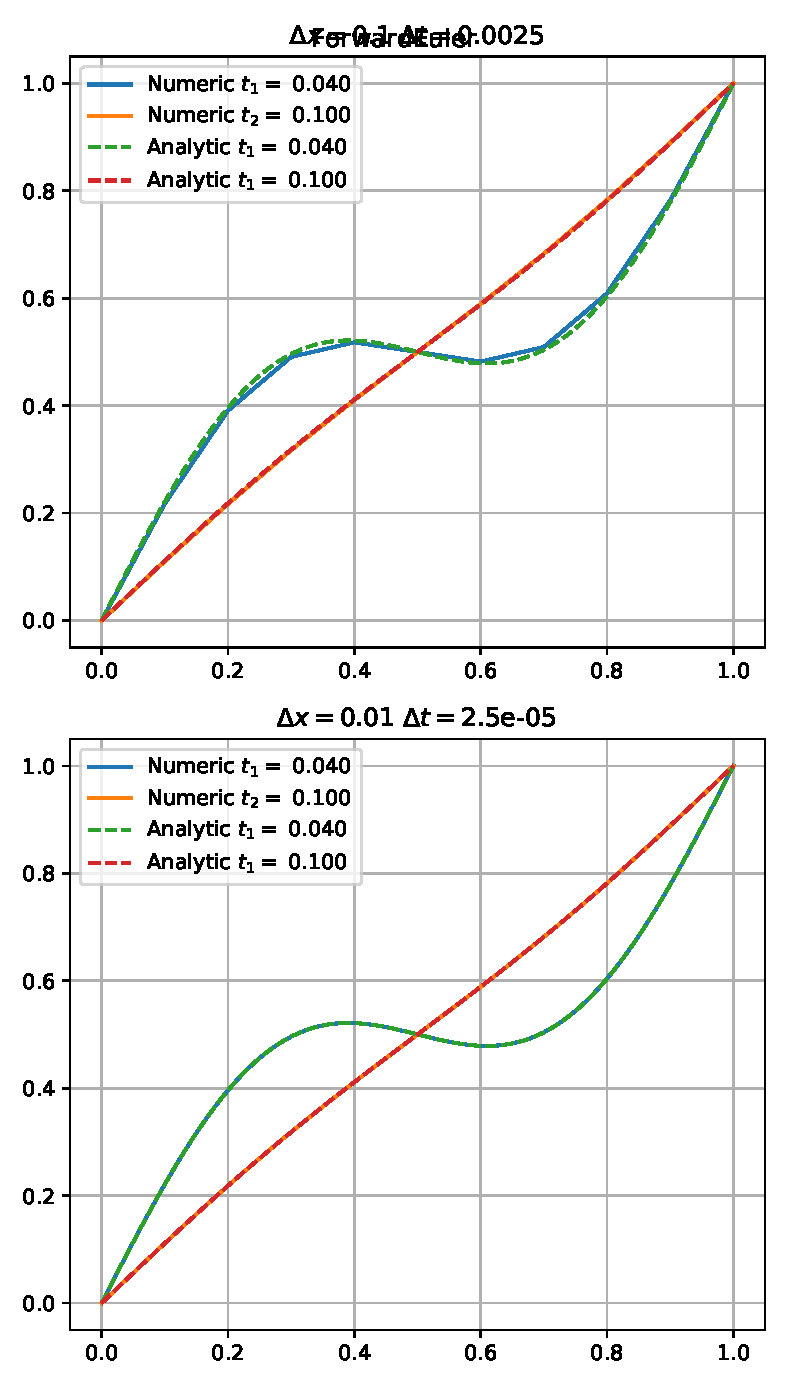
\includegraphics[width=\columnwidth]{../data/ForwardEuler.pdf}
\caption{This figure contains plots of solutions to the one-dimensional diffusion equation, both analytical and numerical with the forward Euler based explicit scheme, for two sets of timestep $\Delta t$ and steplength $\Delta x$. For each set of timestep and steplength a separate plot is provided, and the solutions at two points in time are plotted, as indicated by the legend text. All quantities are dimensionless.} \label{fig:forward_euler_solution}
\end{figure}

\begin{figure}[H]
\centering
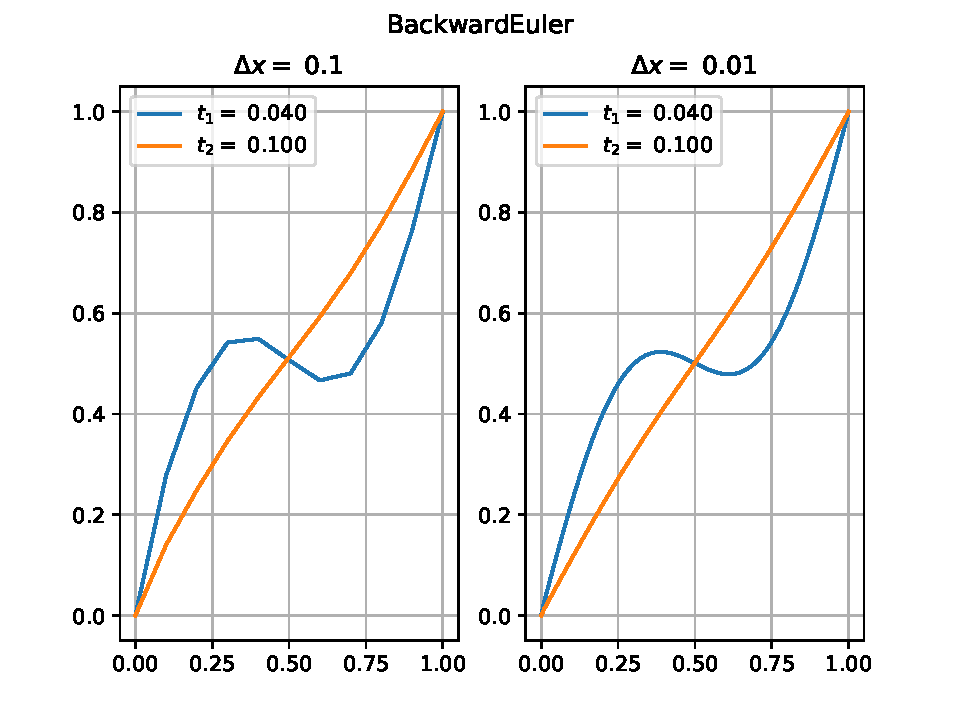
\includegraphics[width=\columnwidth]{../data/BackwardEuler.pdf}
\caption{This figure contains plots of solutions to the one-dimensional diffusion equation, both analytical and numerical with the backward Euler based implicit scheme, for two sets of timestep $\Delta t$ and steplength $\Delta x$. For each set of timestep and steplength a separate plot is provided, and the solutions at two points in time are plotted, as indicated by the legend text. All quantities are dimensionless.} \label{fig:backward_euler_solution}
\end{figure}

\begin{figure}[H]
\centering
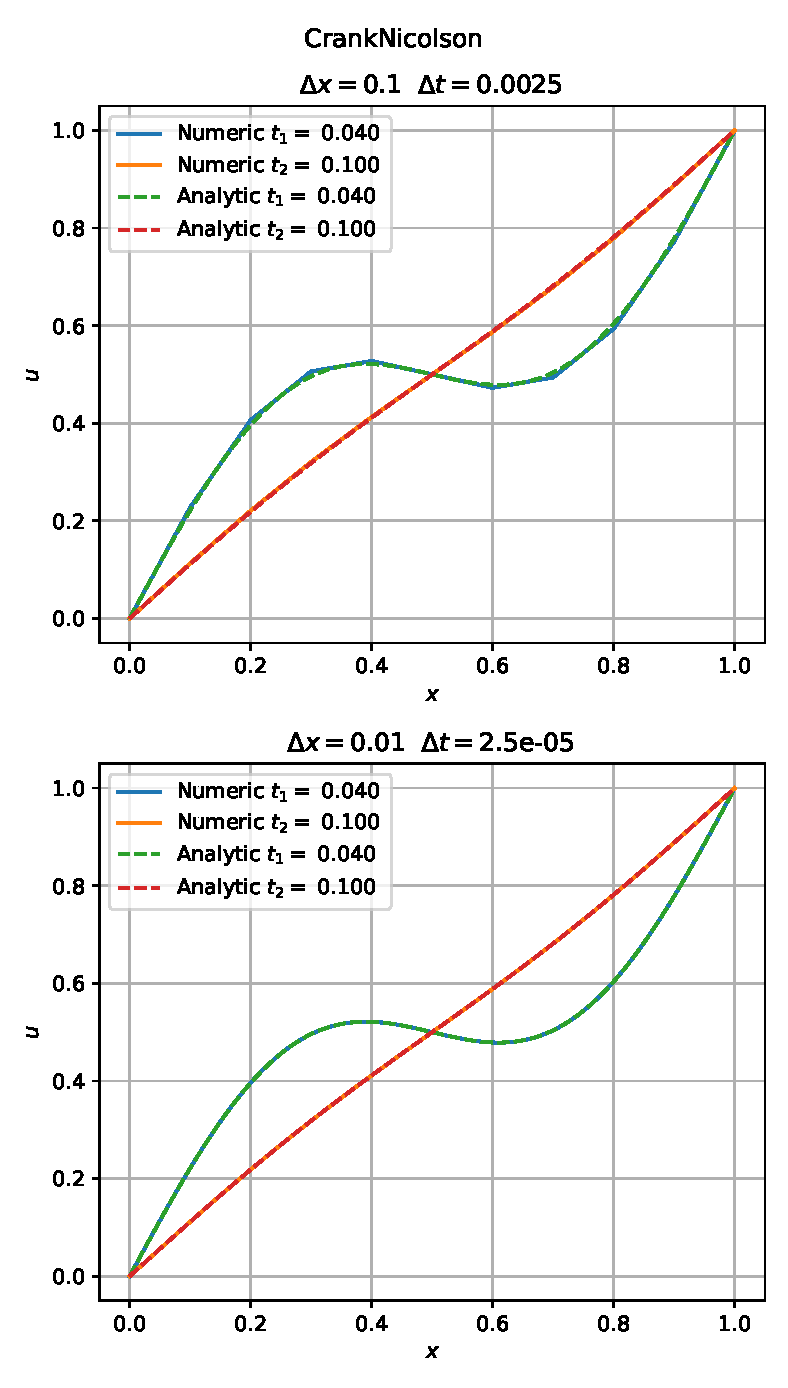
\includegraphics[width=\columnwidth]{../data/CrankNicolson.pdf}
\caption{This figure contains plots of solutions to the one-dimensional diffusion equation, both analytical and numerical with the Crank-Nicolson scheme, for two sets of timestep $\Delta t$ and steplength $\Delta x$. For each set of timestep and steplength a separate plot is provided, and the solutions at two points in time are plotted, as indicated by the legend text. All quantities are dimensionless.} \label{fig:crank_nicolson_solution}
\end{figure}

\begin{figure}[H]
\centering
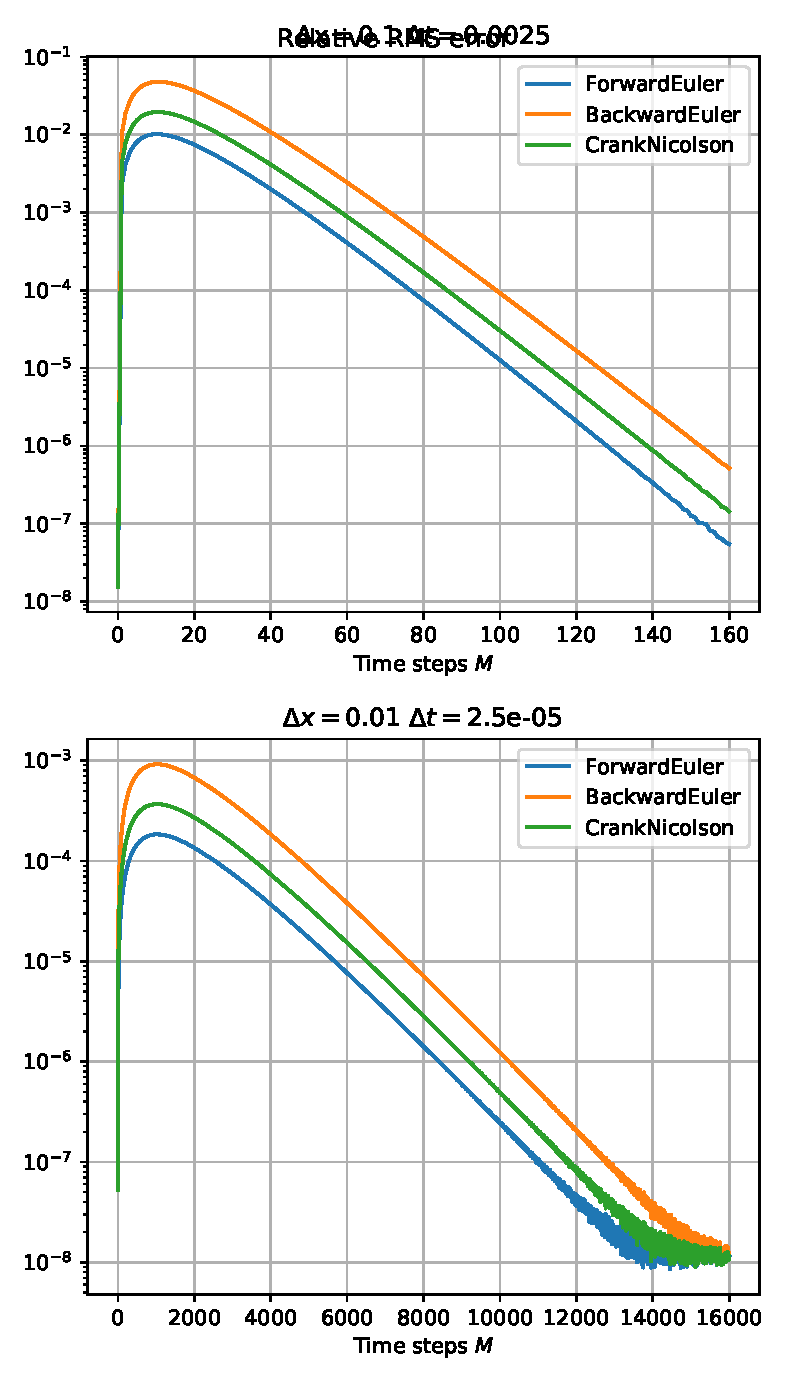
\includegraphics[width=\columnwidth]{../data/1D-RMS.pdf}
\caption{This figure contains plots of the relative RMS error as a function of time against the amount of timesteps for two sets of timestep $\Delta t$ and steplength $\Delta x$ as indicated by the plot titles. The relative RMS error is calculated as in equation \eqref{eq:error_1D}. Each plot contains curves for each of the three numerical schemes outlined in Section \ref{sec:formalism_numerical_1D}, as indicated by the legend text.} \label{fig:error_1D}
\end{figure}

\subsection{Two-dimensional simulation} \label{sec:results_2D}

We solved the two-dimensional dimensionless diffusion equation \eqref{eq:2D_diffusion_equation} numerically, and compared our results with the analytical solution. The intial state, boundary conditions, and analytical solution (equation \eqref{eq:analytical_2D}) are all given in Section \ref{sec:method_2D_sim}. We have plotted the numerical solution at $t=0$, and $t=0.5$ in Figure \ref{fig:solution_2D}. The timestep in this simulation was set to $\Delta t = \num{1e-4}$, and the steplength (both in $x$- and $y$-directions) was set to $h = 0.01$. The relative RMS error (equation \eqref{eq:error_2D}) as a function of time was also plotted against the amount of timesteps. This plot is shown in Figure \ref{fig:error_2D}.

\begin{figure}[H]
\centering
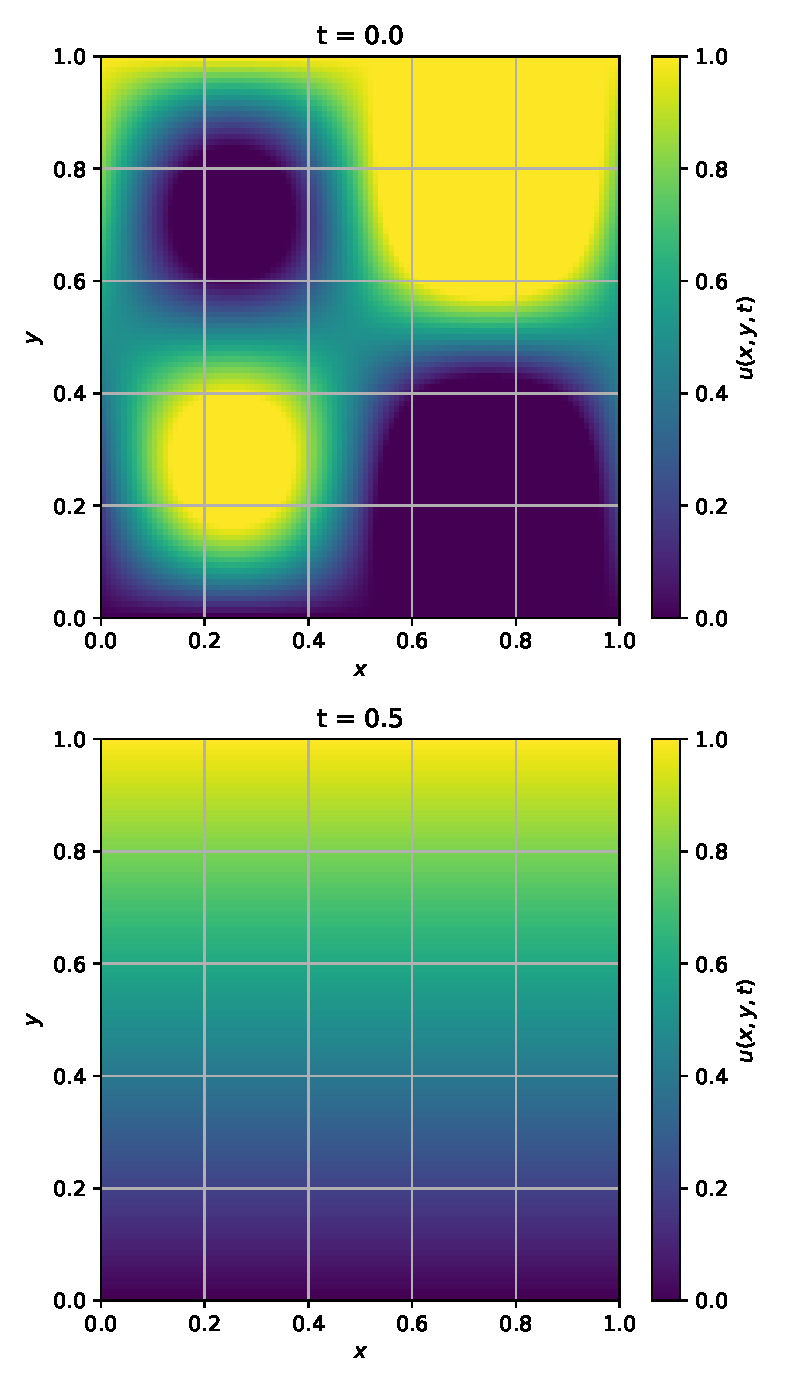
\includegraphics[width=\columnwidth]{../data/2D.pdf}
\caption{This figure contains plots of the initial state in the two-dimensional simulation and numerical solution after a certain amount of time has passed. The first plot shows the initial state, and the second plot shows the numerical solution after a time $t$ specified in the plot title. The timestep in this simulation was $\Delta t = \num{1e-4}$ and the steplength was $h = 0.01$. All quantities in the plots are dimensionless.} \label{fig:solution_2D}
\end{figure}

\begin{figure}[H]
\centering
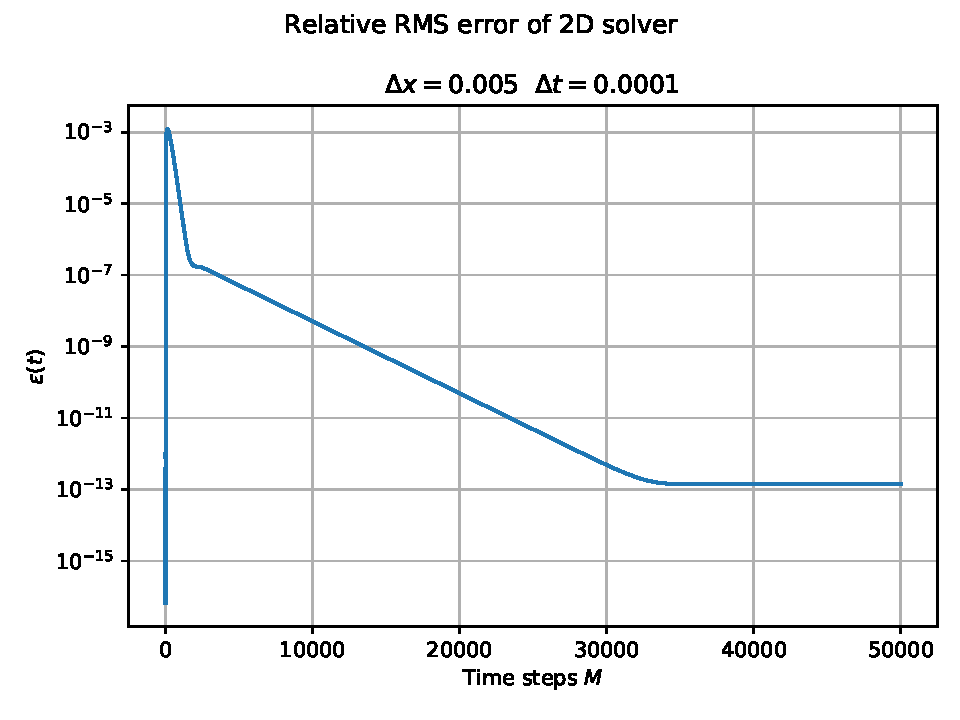
\includegraphics[width=\columnwidth]{../data/2Derr.pdf}
\caption{This figure contains a plot of the relative RMS error (see equation \eqref{eq:error_2D}) as a function of time plotted against the amount of timesteps in the two-dimensional simulation. The timestep $\Delta t$ and steplength $h$ used is indicated in the title of the plot. All quantities in the plot are dimensionless.} \label{fig:error_2D}
\end{figure}

\subsection{Temperature gradient of lithosphere} \label{sec:results_lithosphere}

We simulated the temperature gradient of the lithosphere using our two-dimensional solver. This equates to solving the heat equation with a source term \eqref{eq:heat_eq_with_source_term}. In this section we assume that the reader has read Section \ref{sec:formalism_heat_source_model}. All simulations were run with $N+1 = 101$ grid points in the spatial dimensions and a timestep of $\Delta t = 1e-4$ Gy. 

We estimated the second-order polynomial $p(y)$ as discussed in Section \ref{sec:method_heat_sim}, and used this as the boundary conditions for further simulations. We found:

\begin{align*}
p(y) &= -\frac{439.46}{120^2} \, \frac{\text{K}}{\text{km}^2} \cdot y^2 + \frac{1634.21}{120} \, \frac{\text{K}}{\text{km}} \cdot y + 81.40 \, \text{K} \, ,
\end{align*}

and in order to showcase the fact that the numerical solution is not stable in $x$ with the boundary conditions as dictated by the steady-state solution with no heat sources \eqref{eq:steady_state_heat}, we have included a plot of the first "iteration" of these simulations in Figure \ref{fig:lithosphere_steady_state_project}.

We then ran simulations with the boundary conditions being $T(0,y) = T(1,y) = p(y)$, and the other boundary conditions being the same as before. First a simulation was ran with these boundary conditions with the initial state being the steady state with no heat sources \eqref{eq:steady_state_heat} until the numerical solution had stabilized. We then used the final result from this simulation as the initial state when the heat sources include the further enrichment from the melting sediments \eqref{eq:refertilized_heat}, and simulated this for $1$ Gy. The initial and final states of these two simulations can be seen in Figures \ref{fig:lithosphere_before_enrichment} and \ref{fig:lithosphere_after_enrichment} respectively. 


\begin{figure}[H]
\centering
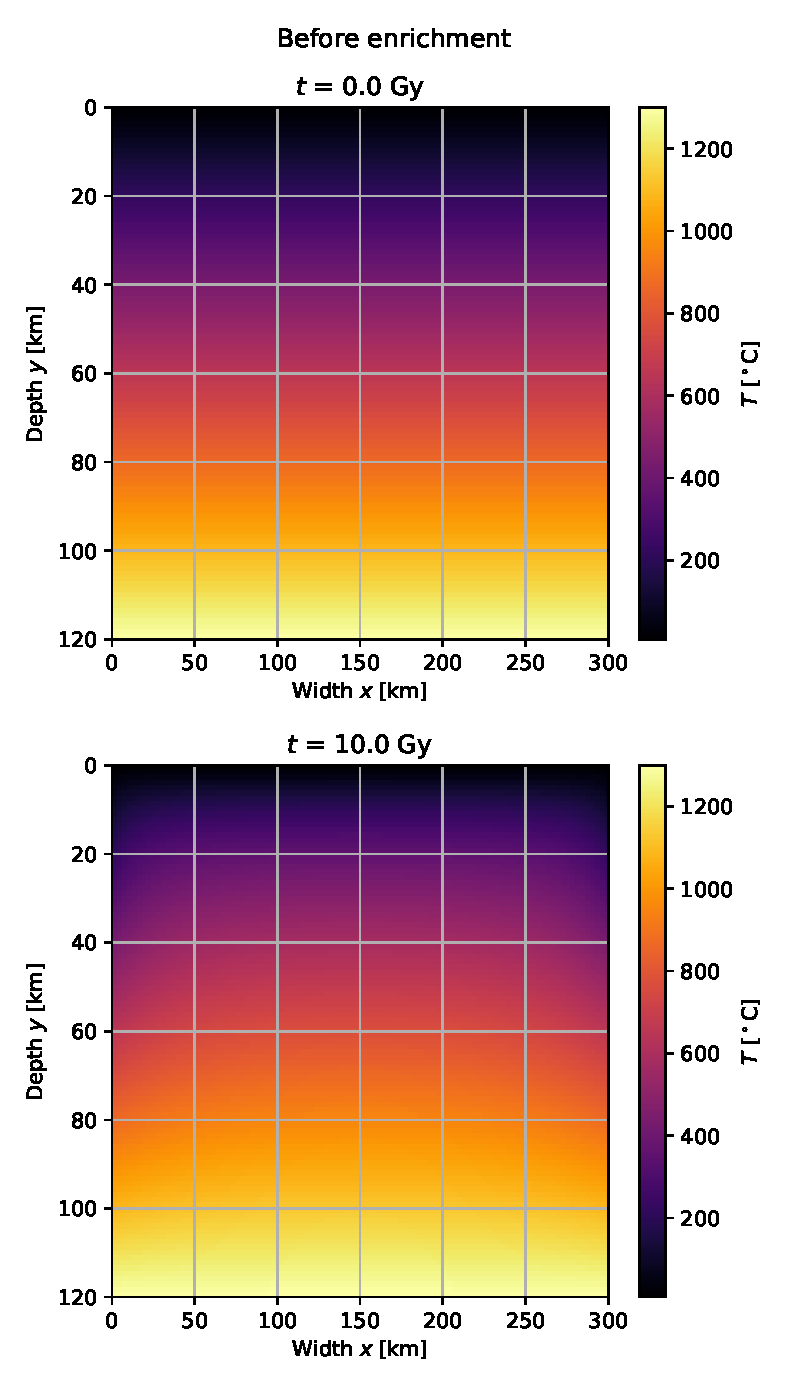
\includegraphics[width=\columnwidth]{../data/2D_first_heat_before.pdf}
\caption{This figure shows the simulated heat gradient of the lithosphere before further radioactive enrichment from the melting of subducting oceanic crust. This simulation uses the boundary conditions derived from the steady-state solution with no added heat. Further details on this system can be found in Sections \ref{sec:formalism_heat_source_model} and \ref{sec:method_heat_sim}. The temperature is marked by the color of the plot as indicated by the colorbar. Units are as shown in the plots. The first plot shows the initial state of the system, and the second plot shows the system after a time of $10$ Gy has passed. } \label{fig:lithosphere_steady_state_project}
\end{figure}


\begin{figure}[H]
\centering
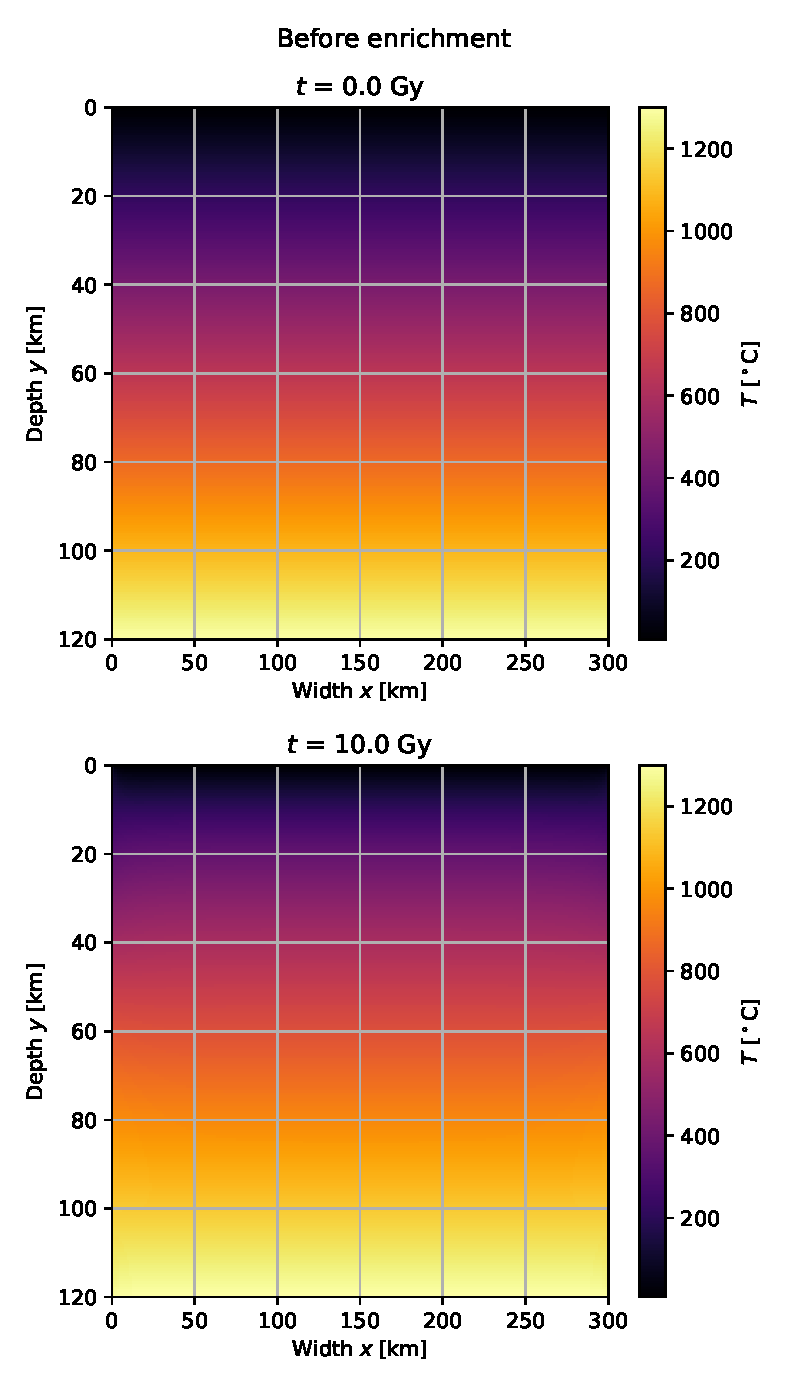
\includegraphics[width=\columnwidth]{../data/2D_heat_before.pdf}
\caption{This figure shows the simulated heat gradient of the lithosphere before further radioactive enrichment from the melting of subducting oceanic crust. This simulation uses the boundary conditions that were found from estimating the steady state solution with added heat from radioactive materials. Further details on this system can be found in Sections \ref{sec:formalism_heat_source_model} and \ref{sec:method_heat_sim}. The temperature is marked by the color of the plot as indicated by the colorbar. Units are as shown in the plots. The first plot shows the initial state of the system, and the second plot shows the system after a time of $10$ Gy has passed.} \label{fig:lithosphere_before_enrichment}
\end{figure}

\begin{figure}[H]
\centering
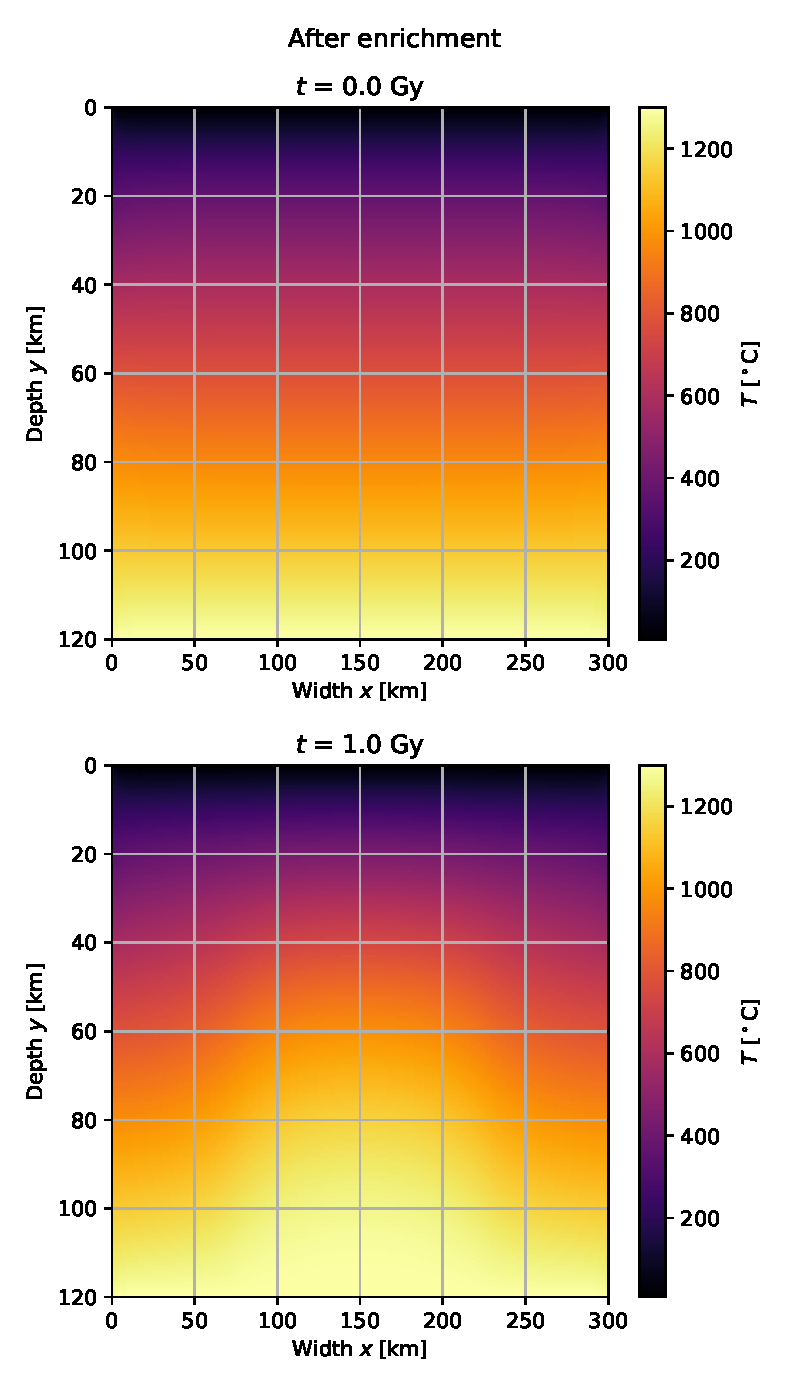
\includegraphics[width=\columnwidth]{../data/2D_heat_after.pdf}
\caption{This figure shows the simulated heat gradient of the lithosphere after further radioactive enrichment from the melting of subducting oceanic crust. Further details on this system can be found in Sections \ref{sec:formalism_heat_source_model} and \ref{sec:method_heat_sim}. The temperature is marked by the color of the plot as indicated by the colorbar. Units are as shown in the plots. The first plot shows the initial state of the system, and the second plot shows the system after a time of $1$ Gy has passed.} \label{fig:lithosphere_after_enrichment}
\end{figure}


\clearpage

\section{Discussion} \label{sec:discussion}

\subsection{Benchmark} \label{sec:discussion_benchmark}
We see from the benchmark results listed in table \ref{table:benchmark} that the forward Euler method is the fastest of the 1D solver methods. By comparison, the backward Euler and Crank-Nicolson are approximately one order of magnitude slower, with the Crank Nicolson method being the slowest of the 1D solver methods. This is what we expected to see given the FLOP counts listed in table \ref{table:FLOPs_1D}.

From table \ref{table:benchmark} we also see that the 2D solver is slower than the 1D solvers by at least three orders of magnitude, something which is expected given the amount of FLOPs needed goes as \(\mathcal{O}(MN^{2})\) (see section \ref{sec:method_2D_solver}) where \(N\) is the number of steps minus one along each axis, and \(M\) is the number of steps in time.

The 2D solver could be further optimized by parallelizing the for-loops that iterate over the matrix elements for each Jacobi iteration, since each element only depends on the state of the matrix in the previous iteration. However, our simple attempts at such a parallelization using OpenMP gave less than satisfactory results, as our solver became significantly slower. At first we assumed the slowdown to be due to the overhead of starting and stopping the parallel region, which occurs once for each Jacobi iteration every time step. To combat the diminishing returns from overhead, we would require a large amount of grid-points in space, and relatively few steps in time. Attempting the parallelized simulation with only one time-step however, was still significantly slow. We assume therefore that our attempt at parallelization was hindered by some other problem, such as false sharing etc.. Due to time constraints, we had to leave the task of parallelization to future research. 

\subsection{One-dimensional simulations} \label{sec:discussion_1D}

We ran simulations with our one-dimensional solver with the same initial and boundary conditions and two sets of steplength $\Delta x$ and timestep $\Delta t$ for all three of the schemes outlined in Section \ref{sec:formalism_numerical_1D}. The results can be seen in Figure \ref{fig:forward_euler_solution} for the forward Euler based scheme, in Figure \ref{fig:backward_euler_solution} for the backward Euler based scheme and in Figure \ref{fig:crank_nicolson_solution} for the Crank-Nicolson scheme. The steplength was chosen so as to be $\Delta x = 0.1$ and $\Delta x = 0.01$ (dimensionless), and the steplength was chosen to be $\Delta t = \Delta x/4$ (also dimensionless), which is within the stability limit of the forward Euler based scheme (see Table \ref{table:schemes_conv_and_err_1D}). The initial state, boundary conditions and the accompanying analytical solution are as stated in Section \ref{sec:method_1D_sims}.

The plots in these figures contain solutions at two points in time: the initial state and after a time such that the solution is starting to resemble the steady-state solution while not yet being perfectly linear, with the analytic solution in these timepoints plotted as well. In all these plots we see the behaviour that we expect for the solvers. All the numerical solutions seem closer to the analytic solution when the resolution (in both time and space) is better, and they also converge similarly with the analytic solution to the steady-state solution. This seems to indicate that the solvers work as they should. 

We also calculated the relative RMS error \eqref{eq:error_1D} in all the three numerical solutions compared to the analytical solution. These results are shown in Figure \ref{fig:error_1D}. Here we see in for both choices of timestep that the error is largest with the backward Euler based scheme, less with the Crank-Nicolson scheme and the least with the forward Euler based scheme. The initial state used was chosen such that the analytical solution is simple. This can clearly be seen in the plots as the error is very small initially as we do not need to approximate the analytical solution, and then starts growing as we start making approximations in order to move the numerical solution ahead in time. For all three schemes we can see that they reach a maximum after roughly the same amount of time, before they dip back and start to tend towards smaller values again. We expect the truncation errors from the approximations and the FLOPs to add up over time when the change is large. However, as both the numerical and analytical solutions approach the steady-state solution, we also expect that the differences between these will decrease, as they should converge towards the same final state. Thus this behaviour is wholly as expected. 

The error also seems to decay faster when the resolution is better, which makes sense. The trunction errors from the approximations will add up and reach a peak as we discussed earlier, and if the resolution is worse, the truncation error will also be worse as they scale with each other (see Table \ref{table:schemes_conv_and_err_1D} for the truncation errors from all schemes). In the plot with better resolution we can also see that the relative RMS error seems to plateau at a certain point, which probably indicates that the error has moved beyond the precision of the numbers recorded. In these simulations the relative error was calculated in a Python script after the simulation was performed. The numerical solutions generated in C++ are written to file with 8 digits of resolution, and the fact that the error plateaus at around $10^{-8}$ is thus probably only an indication of the precision of the numbers being reached. The noise in the graph can also be attributed to the precision of the numbers, and so it seems very likely that this is what is encountered. This will happen in general, as numbers can never be exactly represented on a computer, but if we chose to write the numbers with a precision pertaining to that of the data-type used (doubles in this case, with between $15$ and $18$ significant digits) we would probably see the error plateauing at a much smaller value. 

The most interesting results that can be obtained from these plots is the fact that the error seems to be the smallest with the forward Euler based scheme, instead of the Crank-Nicolson scheme which was found to have a better truncation error (see Table \ref{table:schemes_conv_and_err_1D}). While this may seem weird at first glance, it is not really something that is wholly unexpected. We also counted the amount of FLOPs necessary to solve the system with each numerical scheme (see Table \ref{table:FLOPs_1D}), and there we found that the Crank-Nicolson requires about three times the amount of FLOPs as the forward Euler based scheme. Thus this increase in error can most likely be attributed to the increased amount of FLOPs when compared to the forward Euler based scheme. We cannot, however, completely rule out the possibility that the error might be a product of a fault in our implementation. The error in the backward Euler based scheme is also significantly larger than the one in the forward Euler based scheme while their truncation errors are the same. Similarly to the Crank-Nicolson scheme, the backward Euler based scheme requires more FLOPs than the forward Euler based scheme, and so this might be the leading cause for difference in the errors. However, as both the Crank-Nicolson scheme and the backward Euler based scheme have significantly larger errors in their numerical solutions, this might also indicate an error in our implementation of the tridiagonal solver. We cannot see any error in the implementation, and finding out whether this is the case would probably require comparisons between these methods (and possibly other methods as well) using other methods of solving, which is something that we leave for future research.

All in all, in terms of the error produced, the explicit scheme fares better than the implicit schemes. The implicit schemes naturally requires more FLOPs to solve, and we generally attribute the increase in error this as we do not see any error in our implementations. Assuming that these results are correct, this indicates that the explicit scheme is the better one to choose. This conclusion is a bit naive, however. As the simulations here are not particularly compuationally expensive, the explicit scheme is clearly better. In certain cases when the spatial resolution needs to be very high, however, the stability condition for the explicit scheme might impose that we need an inordinate amount of timesteps in order to simulate for any significant timescale. In these cases we can instead choose to use an implicit scheme, despite it producing more errors, as they do not impose any constraints on the choice of timestep. This can significantly reduce the computational cost, and if the errors produced are not significant enough to matter, the implicit schemes are clearly the better choice. Thus, we conclude that when choosing which scheme to use it is necessary to factor together the computational cost along with the errors produced, and not look at just the errors produced.    

\subsection{Two-dimensional simulation} \label{sec:discussion_2D}
We ran a simulation using our two-dimensional solver with the boundary and initial conditions specified in section \ref{sec:method_2D_sim} with \(\Delta x = \Delta y = h = 1/100\), \(101\times 101\) grid-points, and \(M = 10000\) time steps with \(\Delta t = 10^{-4}\). The results can be found in \autoref{sec:results_2D}.

\subsection{Temperature gradient of lithosphere} \label{sec:discussion_lithosphere}

\clearpage



\section{Conclusion} \label{sec:conclusion}

\onecolumngrid
\bibliography{kilder.bib}{}
\newpage
\twocolumngrid

\appendix
\section{Source code} \label{A}
All code for this report was written in C++ and Python 3.6, and the complete set of files can be found at:

\url{https://github.com/eivinsto/FYS3150_Project_5.git}.

\cprotect\subsection{temp} \label{A.1}

\clearpage
\section{Selected results} \label{B}
Here is a folder of selected results from running our code.

\url{https://github.com/eivinsto/FYS3150_Project_5/tree/master/data}

\newpage
\section{System specifications} \label{C}
All results included in this report were achieved by running the implementation on the following system:

\begin{itemize}
	\item CPU: AMD Ryzen \(9\) \(3900\)X \\
		- \(12\) cores, \(24\) threads. \\ 
		- \(\SI{3.8}{\giga\hertz}\) base clock. \\
		- \(\SI{4.2}{\giga\hertz}\) all core boost clock. \\
		- \(\SI{4.6}{\giga\hertz}\) single core boost clock. \\
	\item RAM: \(2\times\SI{8}{\giga\byte}\) Corsair Vengeance LPX DDR\(4\) \(\SI{3200}{\mega\hertz}\)
\end{itemize}

\end{document}
